\documentclass{bioinfo}

\usepackage{graphicx}
\usepackage{latexsym}
\usepackage{amssymb}
\usepackage{amsmath}
\usepackage{amsfonts}
\usepackage{amsthm}
\usepackage{url}
\usepackage{graphicx}
\usepackage{subfigure}
\usepackage{rotating}
\usepackage{epsfig}
\usepackage{times}
\usepackage{setspace}
\usepackage{natbib}
\usepackage{epstopdf}
\usepackage{multirow}
\usepackage{verbatim} 
\usepackage{array}
\usepackage{bm}
\usepackage{bbm}
\usepackage[nolists,nomarkers]{endfloat}
\usepackage{color}

\newcommand{\todo}[1]{\textbf{***TODO: #1***}}
\renewcommand{\multirowsetup}{\centering}
\newcommand{\argmax}[1]{\underset{#1}{\operatorname{arg}\,\operatorname{max}}\;}

\copyrightyear{2005}
\pubyear{2013}

\begin{document}
\firstpage{1}

\title[Supplement to Detection of Active TFBSs with the Combination of DNase Hypersensitivity and Histone Modifications]
{Supplement to ``Detection of Active Transcription Factor Binding Sites with the Combination of DNase Hypersensitivity and Histone Modifications''}
\author[Gusm\~{a}o \textit{et~al}]{Eduardo G. Gusm\~{a}o\,$^{1}$, Christoph Dieterich\,$^{2}$, Martin Zenke\,$^{3,4}$ and Ivan G. Costa\,$^{1,5,6,}$\footnote{to whom correspondence should be addressed}}
\address{$^{1}$IZKF Computational Biology Research Group, Institute for Biomedical Engineering, RWTH Aachen University Medical School, Germany.\\
$^{2}$Computational RNA Biology and Ageing, Max Planck Institute for Biology of Ageing, Germany. \\
$^{3}$Department of Cell Biology, Institute for Biomedical Engineering, RWTH
Aachen University Medical School, Germany. \\
$^{4}$Helmholtz Institute for Biomedical Engineering, RWTH Aachen University, Germany. \\
$^{5}$Aachen Institute for Advanced Study in Computational Engineering Science (AICES), RWTH Aachen University, Germany. \\
$^{6}$Center of Informatics, Federal University of Pernambuco, Brazil.
}

\history{Received on XXXXX; revised on XXXXX; accepted on XXXXX}

\editor{Associate Editor: XXXXXXX}

\maketitle

\section{Related Work}
\label{sec:related.work}

Recent studies have attempted to improve the active transcription factor binding site (TFBS)
detection using data that reflect chromatin state. We have categorized them in two
classes: segmentation-based methods and site-centric methods. The former
segments the genome in different regions, including likely TFBSs,
based on cell-specific experimental data. The second uses sequence information to identify
TFBSs and then filters these locations for active sites based on
experimental data. In a higher level, each method has its peculiarities and may
address a particular problem which stems from a specific methodological
framework. In addition, each method may have been evaluated with a different
gold standard. Nevertheless, in this study we have performed a comprehensive
comparison including both segmentation-based and site-centric methods.
Following, we introduce the main competing methods.

In~\cite{won2010}, authors used data from the histone modifications
H3K4me1 and H3K4me3 to detect, respectively, active promoter and
enhancer regions. They propose the use of three state hidden Markov
models (HMMs) to capture dip regions of the characteristic peak-dip-peak
shapes of histone modifications indicative of active {\color{black} promoters}/enhancers. 
An HMM was trained for each histone modification on regions with
high number of reads obtained with chromatin immunoprecipitation followed
by sequencing (ChIP-seq) and high scoring TFBSs and combined in a
mixture model. They could demonstrate on data from embryonic stem cells that
their predictions were superior to any of the sequence based TFBS methods.

The advent of DNase-seq technique, which allows genome-wide detection
of open chromatin regions with high resolution, allowed further
improvements~\citep{boyle2011,pique2011}. In~\cite{boyle2011}, an HMM
was developed to detect footprints in specific DNase I digestion
patterns derived from DNase hypersensitivity (DHS) data. Note that the
footprint definition is analogous to finding the dip in a peak-dip-peak
previously explored by~\cite{won2010}, only the sizes of the peaks
and dips are quite distinct between DHS and histone modification
profiles. To cope with the higher resolution of the DHS signals,
authors used a Savitzky-Golay filter to reduce noise and to estimate the
slope of the DHS signal. The prediction task required a five state
HMM, with specific states to identify the decrease/increase of DHS
signals around the peak-dip-peak region. The HMM was trained on a
supervised approach from a single annotated region.

Furthermore, \cite{neph2012a} used an improved and conceptually simplified
segmentation-based method originally proposed in~\cite{hesselberth2009}.
Briefly, they use a sliding window approach in order to find regions
(6--40 bp) with low DHS counts between regions (3--10 bp) with high
DHS counts. A footprint occupancy score (FOS) is evaluated and used
to determine the most significant putative TFBSs. As in~\cite{boyle2011},
the authors use only DHS data.

A quite distinct methodological approach, termed Centipede, was
proposed in~\cite{pique2011}. Briefly, Centipede consists of scanning
the genome for putative TFBSs, gathering experimental and
genomic information around those regions and using an unsupervised
Bayesian approach to label each retrieved site as `bound' or
`unbound'. The experimental and genomic data used included
DHS and histone modifications ChIP-seq, motif matching
bit-score, sequence conservation and distance to the nearest 
transcription start site (TSS). They used DHS as the main source
of information for their predictions and found that histone
modifications did not have a significant improvement in TFBS detection
for most transcription factors (TFs). Note however, that they use a
statistic that summarized the histone occupancy around the
site of interest, therefore not being able to detect the peak-dip-peak
patterns characteristics of this data~\citep{won2010}.

Lastly, \cite{cuellar2012} proposed a technique to include
DHS and histone modification data as prior probability
in the detection of active TFBSs on a probabilistic
classification approach. This study was also the first comparing
approaches, where they showed that the accuracy of Centipede was
mostly superior to their approach.

Moreover, the search of \emph{de novo} motifs can be greatly enhanced
by looking at more specific TFBSs, i.e. footprints closer and
not much broader than the actual TFBSs. To support this claim
we mention two recent studies. In \cite{kulakovskiy2009}, the authors used
footprints derived from a curation of 201 non-redundant DNase I footprinting
studies in \emph{Drosophila}~\cite{bergman2005} to perform motif discovery.
Such analysis allowed the automatic creation of 41 motifs for \emph{Drosophila},
which were shown to have greater sensitivity than previous models. In \cite{neph2012a}
footprints derived from DHS were used for \emph{de novo} motif finding. According to the
authors, despite the efforts devoted to identify cognate recognition
sequences of DNA-binding proteins, high quality motifs are only available
for a small fraction of the TFs with predicted sequence-specific DNA binding
domain. Their analysis on DHS regions found striking 289 footprint-derived
motifs that were absent from major databases.

\section{Datasets}
\label{sec:datasets}

\subsection{ChIP-seq, DNase-seq and PWMs}

We present in Tables~\ref{tab:dataencode}--~\ref{tab:datapwm.hepg2} a
summary of all the data used in this study, including the cell types
HeLa-S3 and HepG2, which were used only in the empirical analysis
described in Section~\ref{sec:hmm.cell.test}. In Table~\ref{tab:dataencode}
we present all DNase-seq and histone modification ChIP-seq experimental data
used as input for our (and competing) methods. In this table we report
the source lab, UCSC accession number, GEO accession number (if available) and
total number of mapped reads used to create the genomic signal for each data
track and cell type. All data presented in this table was obtained in the
ENCODE repository~\citep{encode2012}.

The Tables~\ref{tab:datapwm.h1hesc}--~\ref{tab:datapwm.hepg2} exhibit all
data used to create de validation datasets. Each table contains information
on TFs, ChIP-seq and position weight matrices (PWMs) for one of the cell types. Each
row contains the source lab and UCSC accession number for the TF ChIP-seq, as well
as the repository and ID number of the PWM used to predict true and false
motif-predicted binding sites (MPBSs) for that particular ChIP-seq data. All
ChIP-seq data presented in these tables were obtained in the ENCODE
repository~\citep{encode2012} and all PWMs were obtained in the repositories
Jaspar~\citep{mathelier2014}, Transfac~\citep{matys2006} and Uniprobe~\citep{robasky2011}.

\subsection{Gold Standard}
\label{sec:tfbs.reduction}

Our gold standard was created based on checking overlapping status
of MPBSs (sequence-based predictions obtained with motif matching)
with cell-specific experimental evidence of binding (ChIP-seq peaks,
i.e. enriched regions). We have observed that previous work used distinct
criteria for definition of thresholds for motif matching and detection of
ChIP-seq peaks~\citep{pique2011,boyle2011,cuellar2012,whitington2009}.
Next, we briefly describe the main points concerning the choice of the
parameters necessary in order to create a gold standard to evaluate the methods.

We obtained all TF ChIP-seq data from ENCODE~\citep{encode2012}. We downloaded
the TF enriched regions (peaks) uniformly processed by ENCODE's Analysis Working
Group (AWG).

Concerning motif matching, we evaluated the use of a fixed bit-score
threshold of $ log_2(10^4) \approx 13.2877 $ as proposed in~\cite{pique2011}
and a False Positive Rate (FPR)-based criteria ($10^{-4}$)~\citep{wilczynski2009}.
The latter uses an approach based on dynamic programming to detect
significant TFBSs. In this scenario, a different threshold
is calculated for each motif by defining the bit-score that corresponds
to a specific motif matching FPR-based threshold in the distribution of
scores of that TF's PWM.

The Tables~\ref{tab:H1hesc.tfbsstats}--~\ref{tab:HepG2.tfbsstats} show
statistics on the number of MPBSs, ChIP-seq peaks and combinations of both, for
all cell types used in this study. These tables present data regarding the
$p$-value selection criterion for peak detection and the two motif matching
cutoffs mentioned. The bit-score of $ 13.2877 $ (always in the top line for
each TF) correspond to \cite{pique2011} motif matching cutoff criterion; while
the varying bit-score at each TF's bottom line correspond to the FPR-based
motif matching cutoff. In all cases, the FPR-based selection criterion results
in greater proportion of ChIP-seq peaks with an underlying MPBS than
the fixed bit-score approach. For instance, only $17.54\%$ of the GABPA peaks
in cell type K562 contain overlapping MPBSs selected using bit-score
approach, while $37.61\%$ of these peaks contain overlapping MPBSs selected
using the FPR-based selection. Therefore, we preferred to use the FPR-based
approach, as the fixed bit-score approach represented overly conservative
predictions (on average, only $27.71\%$ of the peaks had their corresponding motifs).

\section{HMM Experimental Design}
\label{sec:experimental.design}

All parameter selection experiments described in this section were based on data
from cell types H1-hESC and K562; and histone modifications H3K4me1 and H4K4me3
unless otherwise stated. All experiments were performed only on chromosome~1,
which was removed from all further analyses.

\subsection{HMM Inference}
\label{sec:hmm.inference}

All HMM models were trained in 10,000 bp randomly selected regions.
The models based on histone modifications H3K4me3, H3K9ac, H3K27ac
and H2A.Z were trained in the region spanning from 211,428,000 bp to
211,438,000 bp in chromosome 1. This region encloses the promoter of 
the gene RCOR3, which is expressed in all cell types analyzed.
The H3K4me1-based models were trained in the region spanning from 26,942,000 bp to
26,952,000 bp, also in chromosome 1. An inspection on ENCODE tracks on the genome 
browser indicates that this region is distal to any known gene and did not 
display any expression levels in the cell types analyzed.

Here we show an example of a complete set of HMM parameters,
regarding the model trained with DHS + H3K4me3 using data from the
H1-hESC cell type. The Table~\ref{tab:hmmtrans} represents the transition
matrix. Each number represents the probability of performing a
transition from the HMM state in the first column of the entry's
row to the HMM state in the first row of the entry's column. The
Table~\ref{tab:hmmmean} exhibits the emission distribution mean values.
It contains the mean in which each signal type (represented in the columns)
assumes at each state (represented in the rows). Finally, the
Table~\ref{tab:hmmcov} shows all covariance matrices from the emission
distributions. The full covariance matrix is depicted for each state,
in which rows and columns are sorted by the input signals: DNase normalized,
DNase slope, H3K4me3 normalized and H3K4me3 slope.

\subsection{Choices Regarding Scaling Methodology}
\label{sec:hmm.norm.test}

Although the first normalization step (within-dataset) is always used in a local
fashion~\citep{boyle2011}, the second normalization step, i.e. the scaling procedure,
can be performed using either local or global values of the standard deviation and percentile.
The local method is depicted in Eq.~2 (main document), using the same windowing as
the normalization procedure. The global method consists on using a single estimate of
standard deviation and percentile for each cell type.

We have performed an empirical analysis to drive the choice of the scaling
methodology and to test different percentile cutoffs. We created receiver
operating characteristic ({\color{black} ROC-like}) curves {\color{black} (with
true negative rate (specificity) on x-axis, instead of the traditional false
positive rate)} and calculated the area under the {\color{black} ROC-like}
curves (AUCs) using our model with signals generated with either global or
local methodologies combined with either the 96th, 98th or 99th percentiles.

We have created boxplots with the distribution of the differences between the local
and global scaling approaches (Fig.~\ref{fig:norm.type}A) and between the different
percentiles tested (Fig.~\ref{fig:norm.type}B). The distributions show a slight
advantage for the local approach and for higher percentile values. Concerning the
choice of percentile, both 98th and 99th percentiles are superior to the 96th
percentile. We chose to use 98th percentile as it presents a more lenient criteria. 

Loosely speaking, using the 98th percentile means that only the top 2$\%$ values
will have a value greater than $0.5$, since the scaling follows a logistic function.
This is supported by estimates of the average coverage of DHS sites or regions enriched
with histone marks over multiple cell types in human genome~\citep{encode2012}
(see Table~\ref{tab:coverage}). See Fig.~\ref{fig:normslope} for example of normalized
and slope signals using the selected scaling parameters.

\subsection{Alternative HMM Topologies}
\label{sec:hmm.topology.test}

The individual pattern of DHS around active TFBSs generally follows the
peak-dip-peak trend when we consider aligned reads from both strands.
This follows directly from the DHS protocol, wherein the DNase I enzyme
nicks the DNA in loci that can be reached~\citep{crawford2006b,song2010,boyle2011}.
However, although the average histone modifications trend generally presents a very
clear (close to symmetric) peak-dip-peak pattern, there is inherent heterogeneity
within individual \emph{loci} regarding signal magnitude, asymmetry and implicit strand
orientation~\citep{kundaje2012,encode2012}. 

We have therefore evaluated two additional HMM topologies depicted in Fig.~\ref{fig:hmm.topologies}.
The model M2 is an extension of the original model (here denoted as M1) to
account for the histone modification signal asymmetry, i.e. that some DHS
sites have very small signals of active histone modifications
on its downstream or upstream regions. For such, two additional transitions were added (shown
in red) in order to allow the DNase level states to be visited when there are
no histone modification peaks before or after DHS peaks. The
new transition probabilities were estimated taking into account the proportions
of asymmetrical peaks reported in~\cite{kundaje2012}. The model M3 is a
simplification of M1, which performs the predictions of footprints without the
slope signal. In M3, the {\tt UP}, {\tt TOP} and {\tt DOWN} states from M1 are
compressed into one state -- {\tt HIGH} -- which recognizes high levels of DHS
(DNase level state) or high levels of histone modifications (histone level state).
Consequently, the HMM needs only the normalized signal and becomes
bivariate (DHS and histone modifications normalized signals).

We tested these three models and obtained {\color{black} ROC-like} curves for all combinations of
cell types, histones and TFs tested. The Fig.~\ref{fig:hmm.topologies.box} shows
the distribution of the AUC differences between these models. We observe a
slight advantage for M1 when compared to M2 (paired Wilcoxon-Mann-Whitney
$p$-value $ = 2.07 \times 10^{-20} $) and a clear advantage of M1 and M2 over
M3 (paired Wilcoxon-Mann-Whitney $p$-value $ = 4.78 \times 10^{-58} $ and
$ 6.35 \times 10^{-37} $, respectively). 

The possible reason for the good results of M1 in relation to M2 is the fact that the
normalization methodology emphasizes even little increases in histone levels leveraging
the asymmetry issue (see Fig.~\ref{fig:asymmetric}). Furthermore, the poor
performance of M3 in comparison to M1 and M2 indicates that even with more complex
models (4 vs. 2 variables and 8 vs. 4 states, respectively) the slope signal and
the additional states are crucial in the accurate delineation of the footprints.

\subsection{Analysis of HMM decoding algorithm}
\label{sec:hmm.posterior.test}

In addition to the Viterbi algorithm implementation, we have tested the usage
of posterior decoding~\citep{rabiner1989} in order to generate our footprint
predictions. In this case, we assume to be footprints contiguous genomic
coordinates $j$ with
\begin{align}
  P(q_{j} = F \! P \: | \: \mathbf{X}) > P(q_{j} = u \: | \: \mathbf{X}) \; \; \; \; \forall \; \; \; u \neq F \! P,
  \label{eq:posterior}
\end{align}
where $ \mathbf{X} $ is the matrix containing the observations (genomic signal) and
$F \! P$ represents the {\tt FOOTPRINT} state.

We show in Fig.~\ref{fig:posterior.test}A the distribution of the pairwise
AUC difference between predictions generated using the Viterbi method and
posterior decoding. We are able to observe that there is a slight advantage
in using the Viterbi method. Despite the lower AUCs for the posterior decoding,
one advantage of such technique would be to use the HMM posterior probabilities
as priors during operations such as motif matching (similarly as in~\cite{cuellar2012}).
However, as can be seen in Fig.~\ref{fig:posterior.test}B, the posterior probability
of the HMM being in the {\tt FOOTPRINT} state changes drastically from 0 to 1.
Such ``spiky'' distribution would lead to results equivalent to the region filtering approach.

\subsection{Analysis of alternative histone modifications}
\label{sec:hmm.histone.test}

We have performed an empirical test on the predictive power of different
histone modifications. All HMM models receive as input a DHS signal and
one histone signal, which in our test varied among the modifications H3K4me1,
H3K4me3, H3K9ac, H3K27ac and the variant H2A.Z. All these histones signals
are associated to active regulatory regions and are frequently measured in
ChIP-seq studies. We also evaluated the combination of all pairs and triples of histone
signals by simply merging all predicted sites, i.e. performing a union step
and merging all predictions that overlapped. This pairwise combination generates
20 additional prediction sets (10 pairs and 10 triples). Note that extending to further
combinations would deviate from one of the main goals, which is to create
a consistent regulatory map with few genome-wide assays. We evaluated all
the 25 combinations to all cell types and TFs tested.
{\color{black} In this analysis, we combined data from cell
types H1-hESC and K562.}

The Fig.~\ref{fig:signaltype.box} presents the distribution of AUCs for all
histone modification models tested. We can observe that most methods present
the region between the first and third quartiles approximately between $80\%$ and
$95\%$. In order to test the statistical relevance of these differences, we
performed a Friedman-Nemenyi test. The Table~\ref{tab:signaltype.friedman} shows
the histone model ranking in decreasing order and their respective Friedman ranking.
The Table~\ref{tab:signaltype.nemenyi} exhibits the full hypothesis test results,
providing information on which models significantly outperformed others.

Overall, histone triples and pairs significantly outperform single histone models.
Although a few histone triples significantly outperformed some histone pairs, this
result is not as clear as the comparison of these models with individual histone
modifications. We chose to report, in the main text, the results for the models
consisting of the best histone triple (H3K4me1+H3K4me3+H3K9ac -- which we denoted
as DH-HMM(3)) and the best histone pair (H3K4me1+H3K4me3 -- which we denoted as
DH-HMM(2)). Note however that several other combinations would perform similarly well.

{\color{black}
In addition, in order to explore the fact that H1-hESC and K562 cell types have
different chromatin landscapes~\citep{dewit2013}, we have split the analysis presented
in this section by cell type. The Friedman-Nemenyi results can be seen in 
Tables~\ref{tab:signaltype.friedman.sep}--\ref{tab:signaltype.nemenyi.k}.

Interestingly, there are differences on the ranking between
H1-hESC and K562. For instance, given the top seven methods (according to the Friedman ranking)
for H1-hESC, five contained H2A.Z; while three contained such histone variant for K562. Furthermore,
the model consisting of the single histone variant H2A.Z was at the bottom of the ranking in K562, while
the individual model with H3K27ac had the worst AUCs in H1-hESC.
One explanation for this is the fact that some histone modifications have distinct
roles depending of the cellular context. For example, H2A.Z plays an important role in
differentiation in Embryonic Stem Cells (ESCs)~\cite{subramanian2013,hu2012}.
On the other hand, H3K27ac (together with H3K4me1) is known to be associated to
poised enhancers but not active sites in stem cells~\cite{rada2010}.

Note, however, that the difference in the individual Friedman ranking between these two
cell types does not result in significant performance variability. The Friedman-Nemenyi
results show that most three-histone models do not significantly outperform other three-histone models.
The same behavior is true when we consider models with histone pairs or singles. This is
in accordance with the Friedman-Nemenyi results for both cell types combined.
}

\subsection{Application of the DH-HMM models on Different Cell Types}
\label{sec:hmm.cell.test}

The annotation of a certain region with the HMM states is laborious. Consequently, it would be interesting to observe the performance
of models trained with data from distinct cell types.  For such, we have expanded
our set of experiments two new cell types (HeLa-S3 and HepG2) each containing 20 and 21 TFs.

In order to test the previous claim, we have performed a paired Wilcoxon-Mann-Whitney test
to compare the distribution of the AUCs for a given cell type with all four models. In particular,
we are interested to observe if there is a significant decrease in AUC when the model
was not trained with the data at hand. The Fig.~\ref{fig:celltype.test} shows the
results for all models applied to all cell types tested. Each set of four
boxplots represent one of the four models, which was applied to the signal
generated from the cell type labeled on the bottom of the set. Statistical significance
on the pairwise difference between these distributions is represented by the
three-star system.

We can observe in Fig.~\ref{fig:celltype.test} that only in one out of twelve cases
the AUC levels are significantly different ($p$-value $\leq 0.05$). This corresponds
to the HepG2 model, when used to generate footprints in the same cell type and
in K562 cell type. These results suggest that our signal processing and models are
able to robustly perform predictions over different cell types. Consequently, a simple application of
the models already stored in our software tool is sufficient to generate accurate predictions. 

{\color{black}
\subsection{TF-oriented Analysis of AUC Results}
\label{sec:hmm.tf.test}

Although the epigenetic grammar around TFBSs is well-characterized for
a number of factors~\cite{encode2012,neph2012a}, it is not known to which
extent such grammar applies to the great variety of human TF binding properties. 

We have performed two analyses regarding this issue. The first analysis
searches for correlations between our method's performance and features
that describe TF binding affinity. In order to test for associations between
these paired samples we used Pearson's product moment correlation coefficient.
The Fig~\ref{fig:tftest.corr} shows a scatterplot between the PWM's information content
(PWM's IC) and our method's AUC (when using three histone modifications). We have observed
no correlation between these two features (correlation coefficient $\approx −0.0204$).

In the second analysis we tested our method's AUC between different 
TF classes. For that, we obtained the TF classification (TFClass)
from~\cite{wingender2013}. TFClass' scheme categorizes TFs based on the
characteristics of their DNA-binding domains. It comprises six levels
(in decreasing order of magnitude: superclasses, classes, families,
subfamilies, genera and factor species). We have observed that the `class' level
would represent a good balance between the number of TFs we used and
information about the TFs' binding characteristics. All TFs used in this
study were categorized with exception of one (NRF1), which fell into
the category of `Yet Undefined DNA-binding Domains'. We present in
Fig.~\ref{fig:tftest.box} the distribution of our method's AUC given the TF
classes. We performed a pairwise two-sided $t$-test between the classes
with a considerable number of TFs (C2H2 zinc finger factors, basic
leucine zipper factors, basic helix−loop−helix factors (bHLH) and
tryptophan cluster factors). This test showed no $p$-value $\leq 0.1$.

The analyses we performed showed no correlation between our method's
performance, i.e. the ability to recognize the epigenetic grammar for
TF binding and many TF features. In this test comprising 83 TFs, our method
seems not to be affected by characteristics of the TF's DNA binding.
Note however that most classes had very few TFs associated (3 classes
with more than 12 TFs). A larger number of TF ChIP-seq is required for
a more thoroughly investigation.
}

{\color{black}
\subsection{Statistics on Footprints and DHS regions}
\label{sec:stats.fp.dhs}

We performed further analyses to investigate the coverage of footprints
in DHS regions. Note that this study can be performed only on segmentation-based
methods, since site-centric methods do not provide genome-wide footprint
predictions (i.e. their predictions are already based on known protein-DNA
binding affinity information).

It is common to encounter multiple footprints at a single DHS region (hotspot).
Our main assumption (and from recent studies~\citep{neph2012a,jankowski2013,boyle2011})
is that this indicates combinatorial binding. First, we calculated the overlap
between the footprint predictions from the three main segmentation-based methods
and the combination of all ChIP-seq peaks used in this study for cell type K562
(see Table~\ref{tab:footchip}). We observed that $66.12\%$ of the footprints obtained
with DH-HMM (with three histones) are supported by a TF ChIP-seq enriched region
(peak) and that $45.12\%$ of the ChIP-seq peaks are supported by a footprint. It is
not possible to evaluate the validity of ``unsupported'' footprints (i.e. footprint
predictions without overlap with our set of ChIP-seq peaks), as they can arise from
TFs not measured in the ChIP-seq experiments used. However, we point to the fact that
our method covered more ChIP-seq regions than Boyle and Neph method (respectively,
$14.93\%$ and $28.39\%$), which reflect the higher sensitivity of our method.

Moreover, we can perform some further analysis to give an overall picture of combinatorial
binding statistics. For these, we estimated the average number of footprints per DHS region
for all segmentation-based methods in cell type K562. We divided DHS regions according to
their occurrence in proximal and distal regions. In this analysis, promoter regions were
considered as [TSS-1500,TSS+100] where the first point in the interval is always upstream.
We also used results from~\cite{yip2012}, which identified regions with extremely high or
low degrees of co-binding (HOT and LOT, respectively) based on the same TF ChIP-seq data
used in this study. As shown in Table~\ref{tab:avgfoot}, all methods tend to find several
footprints per DHS regions. There was a clear trend in finding more footprints in gene proximal
vs. distal regions and HOT vs. LOT. This fits the definition of HOT and LOT regions and the
expectation that more factors bind on proximal promoter regions~\cite{yip2012}. DH-HMM
tends to predict a moderate number of footprints per DHS region, i.e. more footprints than
Boyle and fewer footprints than Neph. Interestingly, both Boyle and Neph clearly underestimate
the number of footprints in LOT regions, where at least one footprint should be available.
This indicates that these methods fail to annotate footprints in LOT regions.

Furthermore, we investigated the DHS regions that contained at least one footprint and
the ones that did not overlap with footprints in cell type K562. The Table~\ref{tab:dhsfoot}
shows a summary of these regions. We observed that DH-HMM with three histone modifications
missed to annotate a lower number of DHS regions than the competing segmentation-based
methods. Moreover, we observed that $1453 (97.65\%)$ and $1347 (90.52\%)$ regions which
the DH-HMM failed to annotate, also did not contain footprints given Boyle and Neph,
respectively. To get further insights about these regions, we plotted a histogram of
the average DNase-seq read counts inside DHS regions with and without footprints for each
method (Fig.~\ref{fig:dhs.histogram}). The histograms indicate that Boyle and Neph fail to
annotate footprints on regions with lower DNase-seq read counts on average. Also, the right tail of
Boyle's and Neph's DNase-seq read count distribution on DHS regions without footprint extends
slightly further when compared to DH-HMM's. This shows that Boyle and Neph also misses
to annotate a few DHS regions with higher DNase-seq read count average.

Finally, we ran the MEME-ChIP tool~\citep{machanick2011} in the set of DHS
regions without any overlap with the footprint predictions from DH-HMM (with
three histone modifications) in order to verify if there are motifs enriched
in this region. We report, in Table~\ref{tab:meme.enrichment}, the motif logo,
MEME $e$-value (log likelihood ratio approximation given a $0$-order Markov background
model), percentage of DHS regions that contained such motif (hits) and the putative
TFs (determined with TOMTOM tool using Jaspar dataset). We report all motifs with an
$e$-value $< 0$. At first glance we observed than only three motifs occurred in more
than $10\%$ of input regions, out of five enriched motifs found. These motifs present
a low number of hits ($33.9\%$, $20.7\%$ and $24.2\%$, sorted increasingly by $e$-value).
The first motif was associated with G rich sequence and eight known TFs. The
second motif could not be associated with any known TF. This indicates that the
DHS regions without footprints have no strong sequence preference. 

}

\section{Experimental Design of Previous Approaches}
\label{sec:experimental.previous.approaches}

\subsection{Boyle et al. Method}
\label{sec:boyle}

The predictions (i.e. footprints) based on \cite{boyle2011} method were
obtained in~\cite{furey2013} for H1-hESC and K562 cell types. They made
available the coordinates of the binding locations, which were used exactly
as reported. In order to make the comparison with our DH-HMM models fair,
we extended their footprints by the same number of base pairs as we extended
the footprints generated with the DH-HMM method (5 bp in each direction).

\subsection{Neph et al. Method}
\label{sec:neph}

For the cell type K562, we obtained the digital genomic footprint predictions
in \cite{neph2012a}, which were used exactly as reported. As footprint predictions
were not available for the cell type H1-hESC, we obtained the scripts and executed
their method with parameters used by the authors in their paper. Briefly, we used
the DHS counts as input with the following parameters: the flanking component length
varied between 3 and 10, and the central footprint region length varied between
6 and 40. Afterwards, the footprints were filtered by the footprint occupancy score
(FOS). As reported in \cite{neph2012a}, a FOS $ \leq 0.95 $ generally agrees with a
false discovery rate (FDR) of $1\%$. All other procedures were executed as described
in \cite{neph2012a}. Additionally, we extended their footprints (both H1-hESC and
K562) by the same number of base pairs as we extended the footprints generated with
the DH-HMM method (5 bp in each direction).

\subsection{Centipede}
\label{sec:centipede}

We obtained the Centipede source code and executed as described
in~\cite{pique2011} for all TFs binding in the cell types H1-hESC and K562.
Briefly, we fetched the DHS signal surrounding a 200 bp window centered
in each motif from our gold standard. The total number of reads within these
regions is modeled as a negative binomial distribution and the spatial
configuration of reads (i.e. the signal at each genomic position) is modelled
as a multinomial (conditional on the total number of reads). Additionally, we
obtained PhastCons conservation score (placental mammals on the 46-way multiple
alignment)~\citep{siepel2005} and Ensembl gene annotation from ENCODE~\citep{hubbard2002}
to create the prior probabilities in addition to the MPBSs bit-score. The latter
is used to generate a signal that corresponds to the distance of every genomic
coordinate to the closest TSS as described in~\citep{pique2011}. Then, we used
the Centipede software to calculate the posterior probabilities of that region
being bound by a TF.

We have noticed that Centipede was very sensitive to the level of shrinkage
of multinomial and negative binomial parameters on a TF/cell type specific way.
Fig.~\ref{fig:centipede.test} shows examples of AUC variation by varying the level
of shrinkage of multinomial and negative binomial parameters from $ 0.0 $ to
$ 1.0 $ by $ 0.5 $. We observe high AUC changes, in the same parameter settings,
when Centipede is applied to distinct TFs. For instance, when the level of
shrinkage of multinomial parameters ($L$) is set to $0.5$ and the level
of shrinkage of negative binomial parameters ($N$) is set to $0.0$ we
observe optimal results for the TFs CTCF and GABPA in cell type H1-hESC
and for TFs CCNT2 and GATA2 in cell type K562. However, for the same
parameters, we observe very low AUCs for TFs Myc and SRF in cell type
H1-hESC and for TFs NF-E2 and TBP in cell type K562. In another example,
when $L$ is set to $1.0$ and $N$ is set to $0.0$, we observe the best AUC
for TFs NF-E2 and TBP but the worst AUC for CCNT2, in cell type K562.
Unfortunately, Centipede framework does not provide a procedure for defining
such parameters.

Therefore, we decided to perform three evaluation scenarios for Centipede.
The first uses the default parameters sugested in~\cite{pique2011}, which corresponds to $L = N = 0.0$
(termed `Default'). The second and third scenarios uses $L$ and $N$ parameters
estimated in a subset of our gold standard, which includes a random sample of
$S$ true MPBSs and $S$ false MPBSs for each TF, where $S$ is the total number
of true MPBSs. In both scenarios, 25 AUCs are calculated for each TF corresponding
to a grid search consisting on the variation of both $L$ and $N$ parameters from
$ 0.0 $ to $ 1.0 $ by $ 0.25 $ intervals. In the second scenario, termed `Estimated',
we use the grid test results (AUCs) to perform a Friedman-Nemenyi hypothesis test
for each cell type in order to estimate the best parameters. Then, we use the
parameters estimated in the cell type K562 for the predictions made in cell type
H1-hESC and vice versa. In the third scenario, termed `Optimistic', we simply use,
for each TF, the parameter settings that generated the best AUC. It is important
to point out that this last TF and cell specific selection criterion is not applicable on a
real scenario, where ChIP-seq experiments for the tested TFs are not available. This 
was performed only to obtain the method accuracies' upper boundaries for
comparison purposes.

The Fig.~\ref{fig:centipede.test.box} shows the AUC distribution based on
all three scenarios discussed previously. In both cell types, the `Default'
model performed poorly than the other two. Also, we observe that the `Estimated'
model AUC distribution is close, but still significantly lower than the `Optimistic'
model AUC distribution ($p$-value $\leq 10^{-5}$ with Wilcoxon-Mann-Whitney test). Interestingly,
the set of parameters estimated in the cell type specific procedure were quite similar 
($L=0.75$ and $N=0$ for H1-hESC and  $L=0.75$ and $N=0.25$ for K562). Our interpretation
is that given our large evaluation set (about 5 times more TFs than in \cite{pique2011}), 
these parameter choices are more robust and should be used as default parameters
to Centipede.

\subsection{Cuellar-Partida et al. Method}
\label{sec:cuellar}

We obtained \cite{cuellar2012} scripts to generate priors and executed
as described in their paper. To create DHS input data,
we evaluated the number of reads aligning to a window of 150 bp,
specified every 20 bp. Histone modification input data was specified in
a 25 bp resolution. In every position, it was summed $ 1 $ if a mapped
read fell within 0--200 bp from the 25 bp window and $ 0.25 $ if it occurred
within 200--300 bp. In order to compare their strategy to ours, priors
were created using, in combination, DHS and histone modifications
H3K4me1+H3K4me3 and H3K4me1+H3K4me3+H3K9a, which we refer as Cuellar(2) and Cuellar(3).

To obtain the predictions, the program FIMO~\citep{grant2011} was used
along with the priors, as suggested by the authors. The establishment of
the motif matching $p$-value threshold led to an issue similar to the
selection of Centipede parameters (Section~\ref{sec:centipede}), i.e. it was
used a selection criteria based on \emph{a posteriori} evaluation of the AUCs
obtained when using different FIMO $p$-value thresholds ($ 10^{-3} $, $ 10^{-4} $,
$ 10^{-5} $, $ 10^{-6} $ and $ 10^{-7} $).

In Fig.~\ref{fig:cuellar.fimo} we can observe that the distribution
of AUCs when FIMO $p$-value $ = 10^{-5}$ is used seems to outperforms all other
thresholds. In order to test this claim, we performed a Friedman-Nemenyi test
on the results of each FIMO $p$-value threshold. By observing the Friedman
ranking and the Friedman-Nemenyi results available in Tables~\ref{tab:cuellarfimo.ranking}
and~\ref{tab:cuellarfimo.fn.auc}, respectively, we are able to define
the FIMO $p$-value $ = 10^{-5}$ as the best choice.

\bibliographystyle{natbib}
\bibliography{document}

%%%%%%%%%%%%%%%%%%%%%%%%
% Figures
%%%%%%%%%%%%%%%%%%%%%%%%

\begin{figure*}[b]
\centering
     \includegraphics[width=0.99\textwidth]{Figs/NormType}
\caption{Scaling parameter grid test. (\textbf{A}) Distribution of the difference between local and global AUCs for all percentile values tested. Positive values indicate the advantage of the local approach. (\textbf{B}) Distribution of the difference between specific percentile values given the local approach. Positive values indicate the advantage of higher percentiles.}
\label{fig:norm.type}
\end{figure*}

\begin{figure*}[b]
\centering
     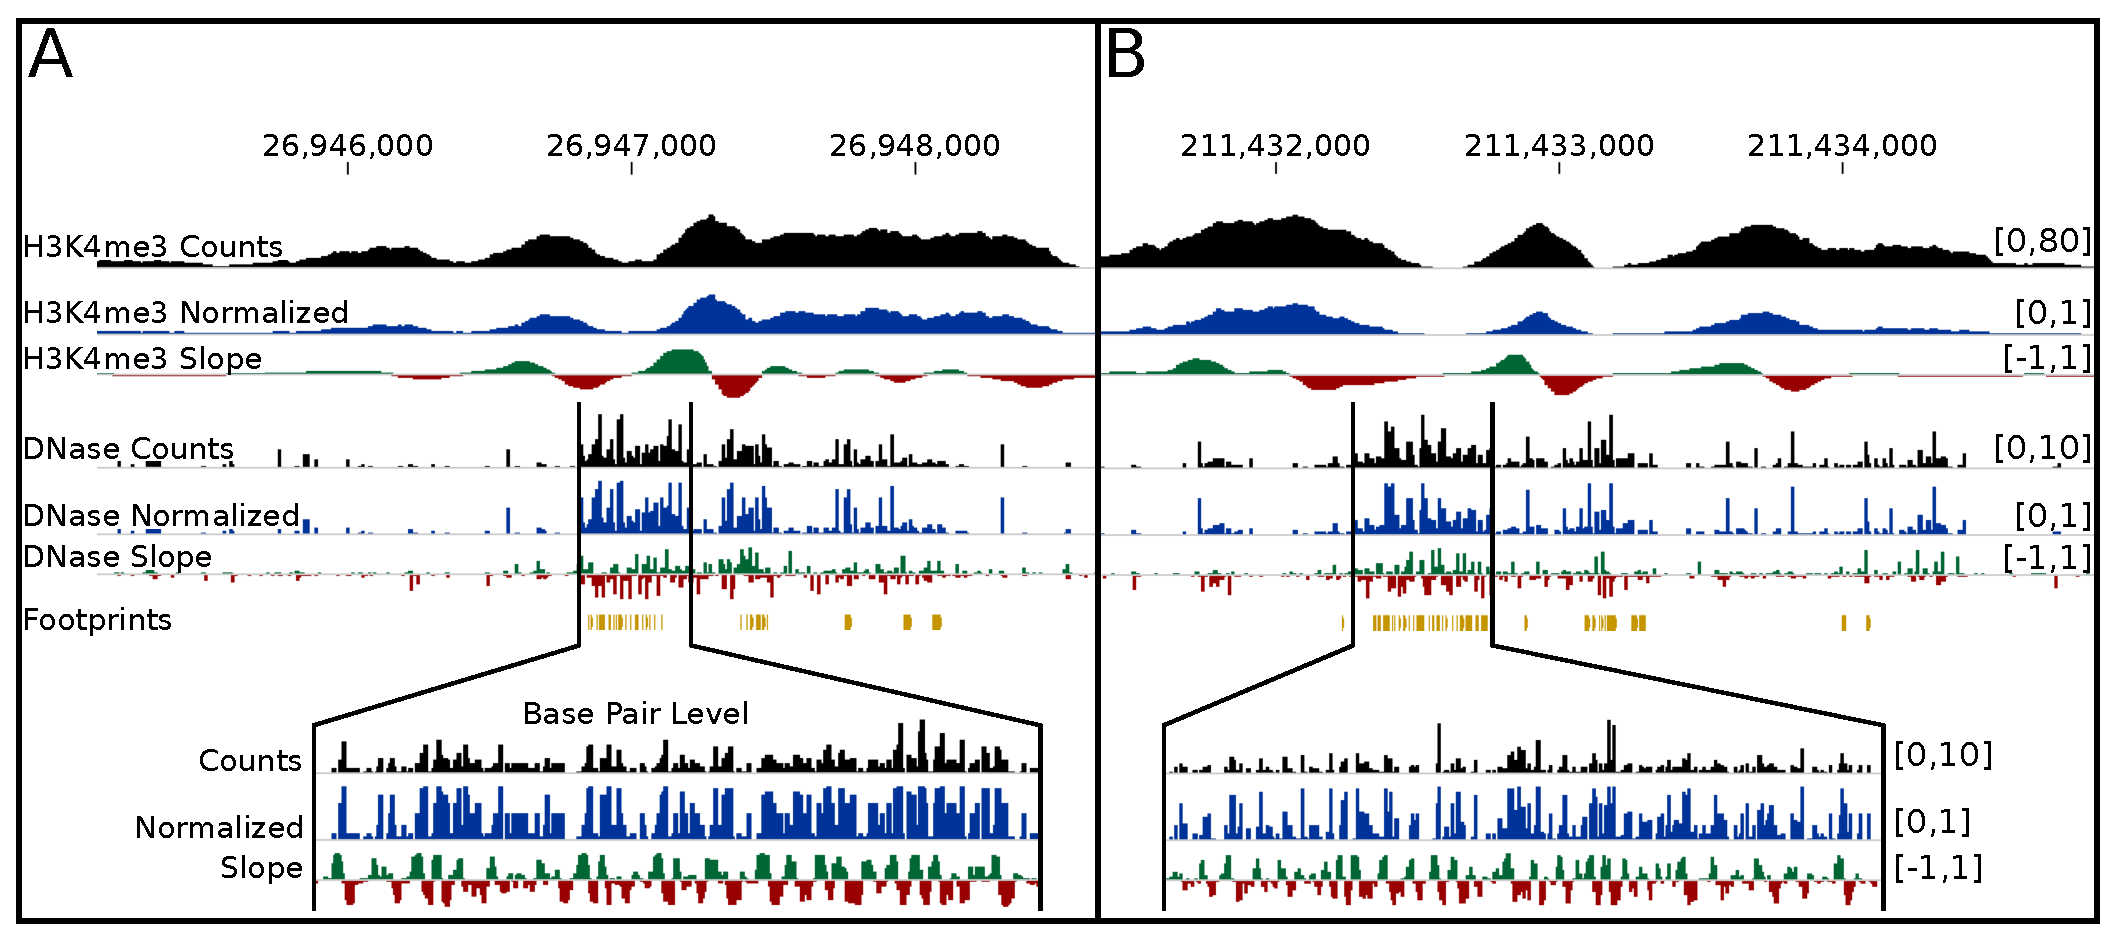
\includegraphics[width=0.99\textwidth]{Figs/NormSlope}
\caption{Example of count, normalized and slope signals for H3K4me3 and DHS for two distinct regions using data from H1-hESC cell type. Signals' ranges can be seen in the right part of the figure.}
\label{fig:normslope}
\end{figure*}

\begin{figure*}[t]
\centering
     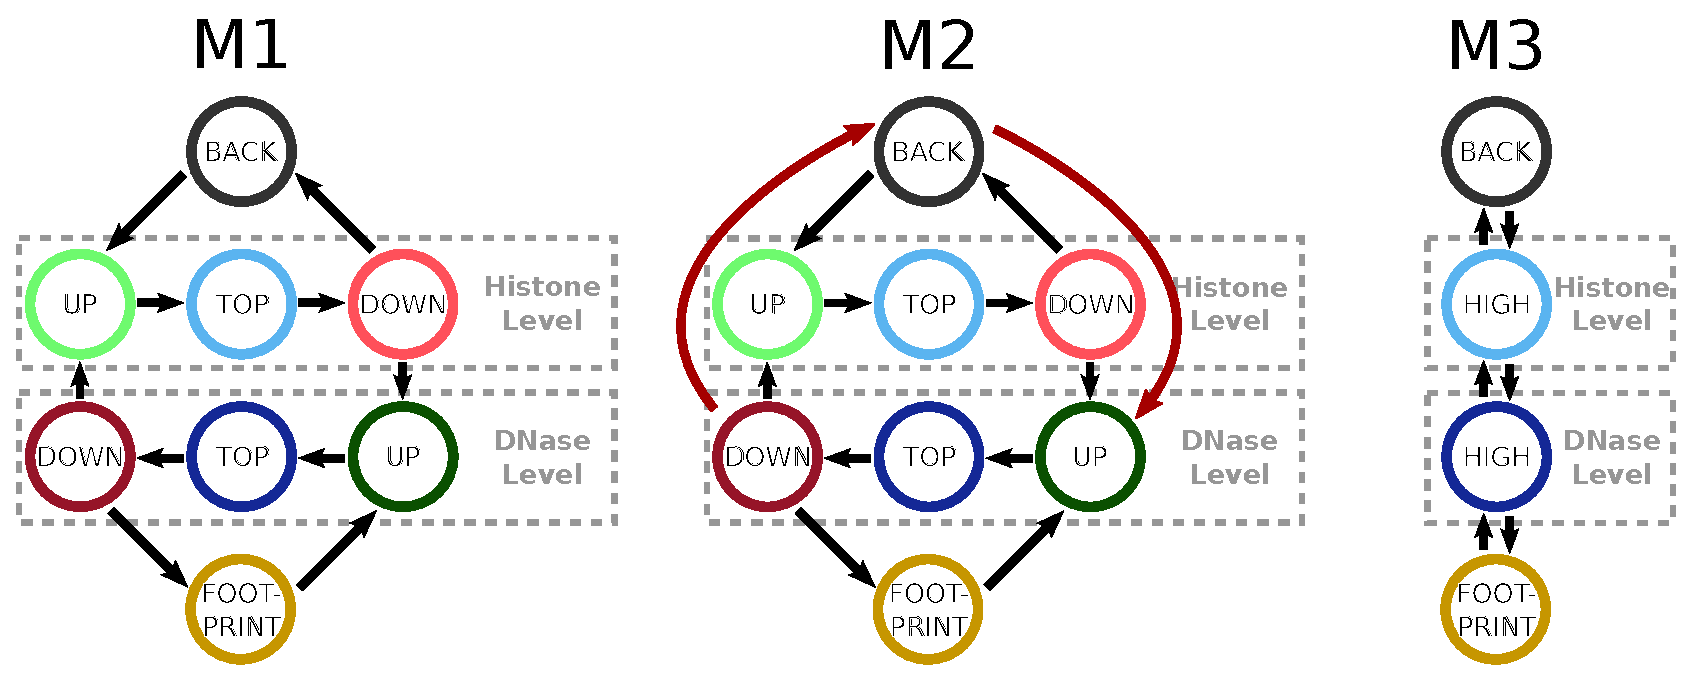
\includegraphics[width=0.99\textwidth]{Figs/HMM_Topologies}
\caption{Depiction of all HMM topologies tested.}
\label{fig:hmm.topologies}
\end{figure*}

\begin{figure*}[t]
\centering
     \includegraphics[width=0.5\textwidth]{Figs/ModelType}
\caption{Distribution of AUC differences between all HMM topologies tested (M1, M2 and M3).}
\label{fig:hmm.topologies.box}
\end{figure*}

\begin{figure*}[t]
\centering
     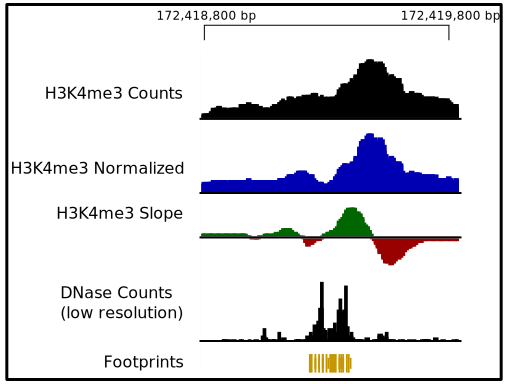
\includegraphics[width=0.5\textwidth]{Figs/Assymetric}
\caption{Example of H3K4me3 count, normalized and slope signals, DHS count signal and footprints predicted in cell type K562 in a region with asymmetrical histone modification profile. Although the leftmost peak from the peak-dip-peak pattern of the H3K4me3 contains very small count signals (very close to the background signal, in this region), the DH-HMM model M1 is still capable of predicting the footprints within the DHS region. Note that after the normalization of the H3K4me3 counts, the resulting signal delineates the DHS region more clearly. We draw the attention to the fact that the DHS signal zooming is such that we are not able to visually identify the footprint signatures.}
\label{fig:asymmetric}
\end{figure*}


\begin{figure*}[t]
\centering
     \includegraphics[width=0.99\textwidth]{Figs/PosteriorTest}
\caption{Viterbi vs. posterior probability test. (\textbf{A}) Distribution of AUC differences between the predictions made using the Viterbi algorithm and the posterior probability. (\textbf{B}) Distribution of the posterior probability of the HMM being in the state {\tt FOOTPRINT} evaluated in a DHS region in chromosome 1 from 211,431,582 to 211,434,492 bp.}
\label{fig:posterior.test}
\end{figure*}


\begin{figure*}[t]
\centering
     \includegraphics[width=0.99\textwidth]{Figs/SignalTypeTest_boxplot}
\caption{Distribution of AUCs for all histone modification models tested. Boxplots are sorted in decreasing order according to their median. Models representing histone triples, pairs and singles are colored in green, blue and red, respectively.}
\label{fig:signaltype.box}
\end{figure*}

\begin{figure*}[t]
\centering
     \includegraphics[width=0.99\textwidth]{Figs/CellType}
\caption{Distribution of AUCs for all HMM models (top x-axis labels) and applied to all cell types (bottom x-axis labels). The first boxplot within each set represents the model trained in the same cell type as the one it was applied to. Statistical significance on the pairwise difference between these distributions is represented by the three-star system.}
\label{fig:celltype.test}
\end{figure*}

%%%

\begin{figure*}[t]
\centering
     \includegraphics[width=0.99\textwidth]{Figs/TfQuality_Correlation}
\caption{{\color{black} Correlation between our method's AUC for DH-HMM(3) and the PWM's IC. Labels with each TF's name are shown with `(H)' for factors binding in H1-hESC and `(K)' for factors binding in K562. The HMM models were trained in the same cell type they were applied. The thicker line in the scatterplot represents the regression line.}}
\label{fig:tftest.corr}
\end{figure*}

\begin{figure*}[t]
\centering
     \includegraphics[width=0.99\textwidth]{Figs/TfQuality_Boxplot}
\caption{{\color{black} Distribution of AUCs for our method (with three histone modifications) categorized by TF class (using TFClass). Below each category's label in the x-axis we show the number of TFs that belong to that class. The boxplot is sorted decreasingly by the number of the TFs in each class.}}
\label{fig:tftest.box}
\end{figure*}

\begin{figure*}[t]
\centering
     \includegraphics[width=0.33\textwidth]{Figs/DHS_Histogram_Boyle}
     \includegraphics[width=0.33\textwidth]{Figs/DHS_Histogram_Neph}
     \includegraphics[width=0.33\textwidth]{Figs/DHS_Histogram_DHHMM3} \\
     \vspace{4mm}
     \includegraphics[width=0.1\textwidth]{Figs/DHS_Histogram_Legend}
\caption{{\color{black} Distribution of the average DNase-seq read counts (in $log_10$ scale) inside DHS regions with/without footprints for the main segmentation-based methods.}}
\label{fig:dhs.histogram}
\end{figure*}

%%%

\begin{figure*}[t]
\centering
     \includegraphics[width=0.99\textwidth]{Figs/CentipedeTest}
\caption{Centipede's {\color{black} ROC-like} curves created for multiple TFs based on a grid variation of Centipede's level of shrinkage of multinomial parameters ($L$) and level of shrinkage of negative binomial parameters ($N$) from $ 0.0 $ to $ 1.0 $ by $ 0.5 $.}
\label{fig:centipede.test}
\end{figure*}

\begin{figure*}[t]
\centering
     \includegraphics[width=0.99\textwidth]{Figs/CentipedeTest_Boxplot}
\caption{Distribution of AUCs for the three scenarios in which Centipede's level of shrinkage of multinomial parameters ($L$) and level of shrinkage of negative binomial parameters ($N$) were defined. `Default' refers to $L = N = 0.0$. `Estimated' refers to parameters estimated on a different cell type. `Optimistic' refers to parameters estimated on the same cell type for each TF individually. Statistical significance on the pairwise difference between these distributions is represented by the three-star system.}
\label{fig:centipede.test.box}
\end{figure*}

\begin{figure*}[t]
\centering
     \includegraphics[width=0.5\textwidth]{Figs/CuellarFimo}
\caption{Distribution of AUCs when using Cuellar's priors with different FIMO $p$-value thresholds.}
\label{fig:cuellar.fimo}
\end{figure*}

%%%%%%%%%%%%%%%%%%%%%%%%
% Tables
%%%%%%%%%%%%%%%%%%%%%%%%

\begin{table*}[t]
\begin{center}
\caption{Friedman ranking. For each metric, the methods are displayed in decreasing order with their respective Friedman ranking.}
\label{tab:ranking}
\renewcommand{\arraystretch}{1.2}
  \begin{tabular}{ |lr|lr|lr| }
    \hline
    \multicolumn{2}{|c|}{\textbf{Sensitivity}} & \multicolumn{2}{|c|}{\textbf{Specificity}} & \multicolumn{2}{|c|}{\textbf{AUC}} \\
    \hline
      Cuellar (2) & 2.2213 & Boyle       & 1.0902 & DH-HMM (3)  & 1.8293 \\
      Cuellar (3) & 2.7459 & Neph        & 2.0082 & DH-HMM (2)  & 2.6707 \\
      DH-HMM (3)  & 3.5    & DH-HMM (2)  & 3.5246 & Centipede   & 4.3902 \\
      Centipede   & 3.5328 & Centipede   & 3.7541 & Neph        & 4.8537 \\
      DH-HMM (2)  & 4.8852 & DH-HMM (3)  & 4.6557 & Cuellar (2) & 5.1098 \\
      H-HMM (3)   & 4.918  & Cuellar (2) & 6.9508 & Cuellar (3) & 5.3293 \\
      H-HMM (2)   & 6.7705 & H-HMM (2)   & 7.1475 & H-HMM (3)   & 6.5732 \\
      Neph        & 7.541  & Cuellar (3) & 7.2623 & H-HMM (2)   & 7.3171 \\
      Boyle       & 8.8852 & H-HMM (3)   & 8.6066 & Boyle       & 7.5    \\
    \hline
  \end{tabular}
\end{center}
\end{table*}

\begin{table*}[t]
\begin{center}
\caption{Transition probabilities of the HMM trained with H3K4me3 using H1-hESC data. Transitions are specified from the states in the rows to the states in the columns. Histone level states are denoted with `(H)' and DNase level states with `(D)'. The {\tt FOOTPRINT} state is abreviated as `FP'.}
\label{tab:hmmtrans}
    \renewcommand{\arraystretch}{1.2}
    \begin{tabular}{ lllllllll }
        \hline
        & \textbf{BACK} & \textbf{UP (H)} & \textbf{TOP (H)} & \textbf{DOWN (H)} & \textbf{UP (D)}
        & \textbf{TOP (D)} & \textbf{DOWN (D)} & \textbf{FP} \\
        \textbf{BACK}     & 0.9997 & 0.0003 & 0.0    & 0.0    & 0.0    & 0.0    & 0.0   & 0.0    \\
        \textbf{UP (H)}   & 0.0    & 0.9915 & 0.0085 & 0.0    & 0.0    & 0.0    & 0.0   & 0.0    \\
        \textbf{TOP (H)}  & 0.0    & 0.0    & 0.9901 & 0.0099 & 0.0    & 0.0    & 0.0   & 0.0    \\
        \textbf{DOWN (H)} & 0.0057 & 0.0    & 0.0    & 0.9861 & 0.0082 & 0.0    & 0.0   & 0.0    \\
        \textbf{UP (D)}   & 0.0    & 0.0    & 0.0    & 0.0    & 0.6515 & 0.3485 & 0.0   & 0.0    \\
        \textbf{TOP (D)}  & 0.0    & 0.0    & 0.0    & 0.0    & 0.0    & 0.783  & 0.217 & 0.0    \\
        \textbf{DOWN (D)} & 0.0    & 0.0339 & 0.0    & 0.0    & 0.0    & 0.0    & 0.577 & 0.3891 \\
        \textbf{FP}       & 0.0    & 0.0    & 0.0    & 0.0    & 0.0564 & 0.0    & 0.0   & 0.9436 \\
        \hline
    \end{tabular}
\end{center}
\end{table*}

\begin{table*}[t]
\begin{center}
\caption{Signals' mean values for each state of the HMM trained with H3K4me3 using H1-hESC data. Histone level states are denoted with `(H)' and DNase level states with `(D)'. The {\tt FOOTPRINT} state is abreviated as `FP'.}
\label{tab:hmmmean}
    \renewcommand{\arraystretch}{1.2}
    \begin{tabular}{ lllll }
        \hline
        & \textbf{DNase norm.} & \textbf{DNase slope} & \textbf{Histone norm.} & \textbf{Histone slope} \\
        \textbf{BACK}     & 0.0045 & -0.0002 & 0.0441 & 0.0007  \\
        \textbf{UP (H)}   & 0.0501 & 0.0043  & 0.1983 & 0.2995  \\
        \textbf{TOP (H)}  & 0.0445 & -0.0075 & 0.4693 & 0.0158  \\
        \textbf{DOWN (H)} & 0.0636 & 0.0003  & 0.2309 & -0.4237 \\
        \textbf{UP (D)}   & 0.1537 & 0.6343  & 0.0894 & -0.0647 \\
        \textbf{TOP (D)}  & 0.4244 & 0.0059  & 0.1091 & -0.0735 \\
        \textbf{DOWN (D)} & 0.1578 & -0.6562 & 0.0816 & -0.0434 \\
        \textbf{FP}       & 0.0902 & -0.0162 & 0.1009 & -0.0436 \\
        \hline
    \end{tabular}
\end{center}
\end{table*}

\begin{table*}[t]
\begin{center}
\caption{Covariance matrices for each state of the HMM trained with H3K4me3 using H1-hESC data. Within each state's matrix, lines and rows are sorted by signal type as DNase normalized, DNase slope, H3K4me3 normalized and H3K4me3 slope. Histone level states are denoted with `(H)' and DNase level states with `(D)'. The {\tt FOOTPRINT} state is abreviated as `FP'.}
\label{tab:hmmcov}
    \renewcommand{\arraystretch}{1.2}
    \begin{tabular}{>{\centering\arraybackslash} m{0.2cm}
                    >{\centering\arraybackslash} m{1.2cm}
                    >{\centering\arraybackslash} m{1.2cm}
                    >{\centering\arraybackslash} m{1.2cm}
                    >{\centering\arraybackslash} m{1.2cm}|
                    >{\centering\arraybackslash} m{0.2cm}
                    >{\centering\arraybackslash} m{1.2cm}
                    >{\centering\arraybackslash} m{1.2cm}
                    >{\centering\arraybackslash} m{1.2cm}
                    >{\centering\arraybackslash} m{1.2cm} }
        \hline
        \multirow{4}{*}{\begin{sideways}\textbf{BACK}\end{sideways}}
        & 0.0025  & -0.0001 & 0.0001 & 0.0    &
        \multirow{4}{*}{\begin{sideways}\textbf{UP (H)}\end{sideways}}
        & 0.0222  & 0.0001  & 0.003  & 0.0057 \\
        & -0.0001 & 0.0025  & 0.0    & 0.0    &
        & 0.0001  & 0.0155  & 0.0006 & 0.0005 \\
        & 0.0001  & 0.0     & 0.0047 & 0.0    &
        & 0.003   & 0.0006  & 0.0101 & 0.0105 \\
        & 0.0     & 0.0     & 0.0    & 0.0019 &
        & 0.0057  & 0.0005  & 0.0105 & 0.0341 \\
        \hline
        \multirow{4}{*}{\begin{sideways}\textbf{TOP (H)}\end{sideways}}
        & 0.0216  & 0.0003  & -0.0009 & 0.0014  &
        \multirow{4}{*}{\begin{sideways}\textbf{DOWN (H)}\end{sideways}}
        & 0.0239  & 0.0001  & -0.0033 & -0.0002 \\
        & 0.0003  & 0.0196  & 0.0005  & 0.0003  &
        & 0.0001  & 0.009   & 0.0002  & -0.0006 \\
        & -0.0009 & 0.0005  & 0.0047  & -0.001  &
        & -0.0033 & 0.0002  & 0.0156  & -0.0095 \\
        & 0.0014  & 0.0003  & -0.001  & 0.0193  &
        & -0.0002 & -0.0006 & -0.0095 & 0.0313  \\
        \hline
        \multirow{4}{*}{\begin{sideways}\textbf{UP (D)}\end{sideways}}
        & 0.0705  & 0.0246  & -0.0053 & 0.0025  &
        \multirow{4}{*}{\begin{sideways}\textbf{TOP (D)}\end{sideways}}
        & 0.1559  & -0.002  & -0.0079 & 0.0052  \\
        & 0.0246  & 0.0714  & -0.0038 & -0.0015 &
        & -0.002  & 0.0384  & -0.0008 & 0.0021  \\
        & -0.0053 & -0.0038 & 0.0045  & -0.0056 &
        & -0.0079 & -0.0008 & 0.007   & -0.0096 \\
        & 0.0025  & -0.0015 & -0.0056 & 0.0125  &
        & 0.0052  & 0.0021  & -0.0096 & 0.0184  \\
        \hline
        \multirow{4}{*}{\begin{sideways}\textbf{DOWN (D)}\end{sideways}}
        & 0.0687  & -0.011  & -0.0048 & 0.004   &
        \multirow{4}{*}{\begin{sideways}\textbf{FP}\end{sideways}}
        & 0.0358  & -0.0019 & -0.0025 & 0.0007  \\
        & -0.011  & 0.055   & 0.0039  & -0.0    &
        & -0.0019 & 0.0225  & 0.0001  & 0.0002  \\
        & -0.0048 & 0.0039  & 0.0039  & -0.0044 &
        & -0.0025 & 0.0001  & 0.0068  & -0.0069 \\
        & 0.004   & -0.0    & -0.0044 & 0.0109  &
        & 0.0007  & 0.0002  & -0.0069 & 0.0121  \\
        \hline
    \end{tabular}
\end{center}
\end{table*}


\begin{table}[t]
\begin{center}
\caption{Coverage of DHS, H3K4me1 and H3K4me3 enriched regions for H1-hESC and K562 cell types.}
\label{tab:coverage}
    \renewcommand{\arraystretch}{1.2}
    \begin{tabular}{>{\raggedright\arraybackslash} m{1.5cm}
                    >{\raggedleft\arraybackslash} m{3.0cm}
                    >{\raggedleft\arraybackslash} m{3.0cm} }
        \hline
        Data Type               & H1-hESC            & K562               \\
        \hline
        DHS                     & 87294396  (2.65\%) & 53487366  (1.62\%) \\
        H3K4me1                 & 16782633  (0.51\%) & 150487948 (4.56\%) \\
        H3K4me3                 & 30857168  (0.94\%) & 71126062  (2.16\%) \\
        H3K4me1+ H3K4me3        & 45289399  (1.37\%) & 174412067 (5.29\%) \\
        DHS+ H3K4me1+ H3K4me3   & 105941410 (3.21\%) & 191774248 (5.81\%) \\
        \hline
    \end{tabular}
\end{center}
\end{table}

\begin{table}[t]
\vspace{0.0cm}
\begin{center}
\caption{Friedman ranking regarding AUC for models based on different histone modification combinations. The models are displayed in decreasing order with their respective Friedman ranking. {\color{black} In this analysis, it was used data from the combination of cell types H1-hESC and K562.}}
\label{tab:signaltype.friedman}
\renewcommand{\arraystretch}{1.2}
  \begin{tabular}{ |lr| }
    \hline
    \multicolumn{2}{|c|}{\textbf{AUC Friedman Ranking}} \\
    \hline
    H3K4me1+H3K4me3+H3K9ac & 3.5568 \\
    H3K4me1+H3K4me3+H3K27ac & 4.8182 \\
    H2A.Z+H3K4me1+H3K4me3 & 5.0341 \\
    H2A.Z+H3K4me3+H3K9ac & 6.4318 \\
    H3K4me3+H3K9ac+H3K27ac & 6.9432 \\
    H2A.Z+H3K4me3+H3K27ac & 7.7841 \\
    H3K4me1+H3K4me3 & 8.625 \\
    H3K4me1+H3K9ac+H3K27ac & 8.8068 \\
    H2A.Z+H3K4me1+H3K9ac & 9.2614 \\
    H3K4me3+H3K9ac & 9.4318 \\
    H2A.Z+H3K4me1+H3K27ac & 10.8409 \\
    H3K4me3+H3K27ac & 11.0795 \\
    H2A.Z+H3K4me3 & 11.5227 \\
    H3K4me1+H3K9ac & 12.0227 \\
    H3K4me1+H3K27ac & 14.3636 \\
    H2A.Z+H3K4me1 & 15.2386 \\
    H2A.Z+H3K9ac+H3K27ac & 15.6705 \\
    H3K4me3 & 16.1932 \\
    H2A.Z+H3K9ac & 18.8864 \\
    H3K9ac+H3K27ac & 18.9545 \\
    H3K4me1 & 19.9432 \\
    H2A.Z+H3K27ac & 20.1364 \\
    H3K9ac & 22.1818 \\
    H3K27ac & 23.5568 \\
    H2A.Z & 23.7159 \\
    \hline
  \end{tabular}
\end{center}
\vspace{0.0cm}
\end{table}

\begin{table}[t]
\vspace{0.0cm}
\begin{center}
\caption{Friedman-Nemenyi hypothesis test results for the AUC metric and the models based on different histone modifications. The asterisk and the cross, respectively, mean that the method in the column outperformed the method in the row with significance levels of 0.05 and 0.1. {\color{black} In this analysis, it was used data from the combination of cell types H1-hESC and K562.}}
\label{tab:signaltype.nemenyi}
\vspace{0.5cm}
\renewcommand{\arraystretch}{1.2}
  \begin{tabular}{ rccccccccccccccccccccccccc }
    & \rotatebox{90}{H3K4me1+H3K4me3+H3K9ac} & \rotatebox{90}{H3K4me1+H3K4me3+H3K27ac} & \rotatebox{90}{H2A.Z+H3K4me1+H3K4me3} & \rotatebox{90}{H2A.Z+H3K4me3+H3K9ac} & \rotatebox{90}{H3K4me3+H3K9ac+H3K27ac} & \rotatebox{90}{H2A.Z+H3K4me3+H3K27ac} & \rotatebox{90}{H3K4me1+H3K4me3} & \rotatebox{90}{H3K4me1+H3K9ac+H3K27ac} & \rotatebox{90}{H2A.Z+H3K4me1+H3K9ac} & \rotatebox{90}{H3K4me3+H3K9ac} & \rotatebox{90}{H2A.Z+H3K4me1+H3K27ac} & \rotatebox{90}{H3K4me3+H3K27ac} & \rotatebox{90}{H2A.Z+H3K4me3} & \rotatebox{90}{H3K4me1+H3K9ac} & \rotatebox{90}{H3K4me1+H3K27ac} & \rotatebox{90}{H2A.Z+H3K4me1} & \rotatebox{90}{H2A.Z+H3K9ac+H3K27ac} & \rotatebox{90}{H3K4me3} & \rotatebox{90}{H2A.Z+H3K9ac} & \rotatebox{90}{H3K9ac+H3K27ac} & \rotatebox{90}{H3K4me1} & \rotatebox{90}{H2A.Z+H3K27ac} & \rotatebox{90}{H3K9ac} & \rotatebox{90}{H3K27ac} & \rotatebox{90}{H2A.Z} \\
    \hline
    H3K4me1+H3K4me3+H3K9ac &     &     &     &     &     &     &     &     &     &     &     &     &     &     &     &     &     &     &     &     &     &     &     &     &     \\
    H3K4me1+H3K4me3+H3K27ac &     &     &     &     &     &     &     &     &     &     &     &     &     &     &     &     &     &     &     &     &     &     &     &     &     \\
    H2A.Z+H3K4me1+H3K4me3 &     &     &     &     &     &     &     &     &     &     &     &     &     &     &     &     &     &     &     &     &     &     &     &     &     \\
    H2A.Z+H3K4me3+H3K9ac &     &     &     &     &     &     &     &     &     &     &     &     &     &     &     &     &     &     &     &     &     &     &     &     &     \\
    H3K4me3+H3K9ac+H3K27ac &     &     &     &     &     &     &     &     &     &     &     &     &     &     &     &     &     &     &     &     &     &     &     &     &     \\
    H2A.Z+H3K4me3+H3K27ac & $*$ &     &     &     &     &     &     &     &     &     &     &     &     &     &     &     &     &     &     &     &     &     &     &     &     \\
    H3K4me1+H3K4me3 & $*$ &     &     &     &     &     &     &     &     &     &     &     &     &     &     &     &     &     &     &     &     &     &     &     &     \\
    H3K4me1+H3K9ac+H3K27ac & $*$ & $+$ &     &     &     &     &     &     &     &     &     &     &     &     &     &     &     &     &     &     &     &     &     &     &     \\
    H2A.Z+H3K4me1+H3K9ac & $*$ & $*$ & $*$ &     &     &     &     &     &     &     &     &     &     &     &     &     &     &     &     &     &     &     &     &     &     \\
    H3K4me3+H3K9ac & $*$ & $*$ & $*$ &     &     &     &     &     &     &     &     &     &     &     &     &     &     &     &     &     &     &     &     &     &     \\
    H2A.Z+H3K4me1+H3K27ac & $*$ & $*$ & $*$ & $*$ & $+$ &     &     &     &     &     &     &     &     &     &     &     &     &     &     &     &     &     &     &     &     \\
    H3K4me3+H3K27ac & $*$ & $*$ & $*$ & $*$ & $*$ &     &     &     &     &     &     &     &     &     &     &     &     &     &     &     &     &     &     &     &     \\
    H2A.Z+H3K4me3 & $*$ & $*$ & $*$ & $*$ & $*$ &     &     &     &     &     &     &     &     &     &     &     &     &     &     &     &     &     &     &     &     \\
    H3K4me1+H3K9ac & $*$ & $*$ & $*$ & $*$ & $*$ & $*$ &     &     &     &     &     &     &     &     &     &     &     &     &     &     &     &     &     &     &     \\
    H3K4me1+H3K27ac & $*$ & $*$ & $*$ & $*$ & $*$ & $*$ & $*$ & $*$ & $*$ & $*$ &     &     &     &     &     &     &     &     &     &     &     &     &     &     &     \\
    H2A.Z+H3K4me1 & $*$ & $*$ & $*$ & $*$ & $*$ & $*$ & $*$ & $*$ & $*$ & $*$ & $*$ & $*$ &     &     &     &     &     &     &     &     &     &     &     &     &     \\
    H2A.Z+H3K9ac+H3K27ac & $*$ & $*$ & $*$ & $*$ & $*$ & $*$ & $*$ & $*$ & $*$ & $*$ & $*$ & $*$ & $*$ &     &     &     &     &     &     &     &     &     &     &     &     \\
    H3K4me3 & $*$ & $*$ & $*$ & $*$ & $*$ & $*$ & $*$ & $*$ & $*$ & $*$ & $*$ & $*$ & $*$ & $*$ &     &     &     &     &     &     &     &     &     &     &     \\
    H2A.Z+H3K9ac & $*$ & $*$ & $*$ & $*$ & $*$ & $*$ & $*$ & $*$ & $*$ & $*$ & $*$ & $*$ & $*$ & $*$ & $*$ &     &     &     &     &     &     &     &     &     &     \\
    H3K9ac+H3K27ac & $*$ & $*$ & $*$ & $*$ & $*$ & $*$ & $*$ & $*$ & $*$ & $*$ & $*$ & $*$ & $*$ & $*$ & $*$ &     &     &     &     &     &     &     &     &     &     \\
    H3K4me1 & $*$ & $*$ & $*$ & $*$ & $*$ & $*$ & $*$ & $*$ & $*$ & $*$ & $*$ & $*$ & $*$ & $*$ & $*$ & $*$ & $*$ &     &     &     &     &     &     &     &     \\
    H2A.Z+H3K27ac & $*$ & $*$ & $*$ & $*$ & $*$ & $*$ & $*$ & $*$ & $*$ & $*$ & $*$ & $*$ & $*$ & $*$ & $*$ & $*$ & $*$ & $+$ &     &     &     &     &     &     &     \\
    H3K9ac & $*$ & $*$ & $*$ & $*$ & $*$ & $*$ & $*$ & $*$ & $*$ & $*$ & $*$ & $*$ & $*$ & $*$ & $*$ & $*$ & $*$ & $*$ &     &     &     &     &     &     &     \\
    H3K27ac & $*$ & $*$ & $*$ & $*$ & $*$ & $*$ & $*$ & $*$ & $*$ & $*$ & $*$ & $*$ & $*$ & $*$ & $*$ & $*$ & $*$ & $*$ & $*$ & $*$ &     &     &     &     &     \\
    H2A.Z & $*$ & $*$ & $*$ & $*$ & $*$ & $*$ & $*$ & $*$ & $*$ & $*$ & $*$ & $*$ & $*$ & $*$ & $*$ & $*$ & $*$ & $*$ & $*$ & $*$ &     &     &     &     &     \\
    \hline
  \end{tabular}
\end{center}
\vspace{0.0cm}
\end{table}

%%%%%%%%%%%%

\begin{table}[t]
\vspace{0.0cm}
\begin{center}
\caption{{\color{black} Friedman ranking regarding AUC for models based on different histone modification combinations. The models are displayed in decreasing order with their respective Friedman ranking. In this analysis, it was used data from the cell types H1-hESC and K562 in separate.}}
\label{tab:signaltype.friedman.sep}
\renewcommand{\arraystretch}{1.2}
  \begin{tabular}{ |lr|lr| }
    \hline
    \multicolumn{2}{|c|}{\textbf{AUC (H1-hESC)}} & \multicolumn{2}{|c|}{\textbf{AUC (K562)}} \\
    \hline
    H2A.Z+H3K4me1+H3K4me3 & 3.5172 & H3K4me1+H3K4me3+H3K9ac & 2.7797 \\
    H3K4me1+H3K4me3+H3K9ac & 5.1379 & H3K4me1+H3K4me3+H3K27ac & 4.5593 \\
    H3K4me1+H3K4me3+H3K27ac & 5.3448 & H3K4me3+H3K9ac+H3K27ac & 5.2542 \\
    H2A.Z+H3K4me1+H3K9ac & 6.6897 & H2A.Z+H3K4me1+H3K4me3 & 5.7797 \\
    H2A.Z+H3K4me1+H3K27ac & 6.7931 & H2A.Z+H3K4me3+H3K9ac & 5.8136 \\
    H2A.Z+H3K4me3+H3K27ac & 7.5172 & H3K4me3+H3K9ac & 7.2034 \\
    H2A.Z+H3K4me3+H3K9ac & 7.6897 & H2A.Z+H3K4me3+H3K27ac & 7.9153 \\
    H3K4me1+H3K9ac+H3K27ac & 8.9655 & H3K4me1+H3K4me3 & 8.4237 \\
    H3K4me1+H3K4me3 & 9.0345 & H3K4me1+H3K9ac+H3K27ac & 8.7288 \\
    H3K4me3+H3K9ac+H3K27ac & 10.3793 & H3K4me3+H3K27ac & 9.6271 \\
    H2A.Z+H3K4me1 & 10.7241 & H2A.Z+H3K4me1+H3K9ac & 10.5254 \\
    H2A.Z+H3K4me3 & 10.931 & H2A.Z+H3K4me3 & 11.8136 \\
    H3K4me1+H3K9ac & 12.3448 & H3K4me1+H3K9ac & 11.8644 \\
    H3K4me1+H3K27ac & 13.3448 & H2A.Z+H3K4me1+H3K27ac & 12.8305 \\
    H2A.Z+H3K9ac+H3K27ac & 13.8966 & H3K4me3 & 14.4746 \\
    H3K4me3+H3K9ac & 13.9655 & H3K4me1+H3K27ac & 14.8644 \\
    H3K4me3+H3K27ac & 14.0345 & H2A.Z+H3K9ac+H3K27ac & 16.5424 \\
    H2A.Z+H3K27ac & 17.2069 & H2A.Z+H3K4me1 & 17.4576 \\
    H2A.Z+H3K9ac & 17.4483 & H3K9ac+H3K27ac & 17.8814 \\
    H3K4me1 & 19.4138 & H2A.Z+H3K9ac & 19.5932 \\
    H3K4me3 & 19.6897 & H3K4me1 & 20.2034 \\
    H3K9ac+H3K27ac & 21.1379 & H3K9ac & 21.3559 \\
    H2A.Z & 21.7586 & H2A.Z+H3K27ac & 21.5763 \\
    H3K9ac & 23.8621 & H3K27ac & 23.2542 \\
    H3K27ac & 24.1724 & H2A.Z & 24.678 \\
    \hline
  \end{tabular}
\end{center}
\vspace{0.0cm}
\end{table}

\begin{table}[t]
\vspace{0.0cm}
\begin{center}
\caption{{\color{black} Friedman-Nemenyi hypothesis test results for the AUC metric and the models based on different histone modifications. The asterisk and the cross, respectively, mean that the method in the column outperformed the method in the row with significance levels of 0.05 and 0.1. In this analysis, it was used data from the cell type \textbf{H1-hESC}.}}
\label{tab:signaltype.nemenyi.h}
\vspace{0.5cm}
\renewcommand{\arraystretch}{1.2}
  \begin{tabular}{ rccccccccccccccccccccccccc }
    & \rotatebox{90}{H2A.Z+H3K4me1+H3K4me3} & \rotatebox{90}{H3K4me1+H3K4me3+H3K9ac} & \rotatebox{90}{H3K4me1+H3K4me3+H3K27ac} & \rotatebox{90}{H2A.Z+H3K4me1+H3K9ac} & \rotatebox{90}{H2A.Z+H3K4me1+H3K27ac} & \rotatebox{90}{H2A.Z+H3K4me3+H3K27ac} & \rotatebox{90}{H2A.Z+H3K4me3+H3K9ac} & \rotatebox{90}{H3K4me1+H3K9ac+H3K27ac} & \rotatebox{90}{H3K4me1+H3K4me3} & \rotatebox{90}{H3K4me3+H3K9ac+H3K27ac} & \rotatebox{90}{H2A.Z+H3K4me1} & \rotatebox{90}{H2A.Z+H3K4me3} & \rotatebox{90}{H3K4me1+H3K9ac} & \rotatebox{90}{H3K4me1+H3K27ac} & \rotatebox{90}{H2A.Z+H3K9ac+H3K27ac} & \rotatebox{90}{H3K4me3+H3K9ac} & \rotatebox{90}{H3K4me3+H3K27ac} & \rotatebox{90}{H2A.Z+H3K27ac} & \rotatebox{90}{H2A.Z+H3K9ac} & \rotatebox{90}{H3K4me1} & \rotatebox{90}{H3K4me3} & \rotatebox{90}{H3K9ac+H3K27ac} & \rotatebox{90}{H2A.Z} & \rotatebox{90}{H3K9ac} & \rotatebox{90}{H3K27ac} \\
    \hline
    H2A.Z+H3K4me1+H3K4me3 &     &     &     &     &     &     &     &     &     &     &     &     &     &     &     &     &     &     &     &     &     &     &     &     &     \\
    H3K4me1+H3K4me3+H3K9ac &     &     &     &     &     &     &     &     &     &     &     &     &     &     &     &     &     &     &     &     &     &     &     &     &     \\
    H3K4me1+H3K4me3+H3K27ac &     &     &     &     &     &     &     &     &     &     &     &     &     &     &     &     &     &     &     &     &     &     &     &     &     \\
    H2A.Z+H3K4me1+H3K9ac &     &     &     &     &     &     &     &     &     &     &     &     &     &     &     &     &     &     &     &     &     &     &     &     &     \\
    H2A.Z+H3K4me1+H3K27ac &     &     &     &     &     &     &     &     &     &     &     &     &     &     &     &     &     &     &     &     &     &     &     &     &     \\
    H2A.Z+H3K4me3+H3K27ac &     &     &     &     &     &     &     &     &     &     &     &     &     &     &     &     &     &     &     &     &     &     &     &     &     \\
    H2A.Z+H3K4me3+H3K9ac &     &     &     &     &     &     &     &     &     &     &     &     &     &     &     &     &     &     &     &     &     &     &     &     &     \\
    H3K4me1+H3K9ac+H3K27ac &     &     &     &     &     &     &     &     &     &     &     &     &     &     &     &     &     &     &     &     &     &     &     &     &     \\
    H3K4me1+H3K4me3 &     &     &     &     &     &     &     &     &     &     &     &     &     &     &     &     &     &     &     &     &     &     &     &     &     \\
    H3K4me3+H3K9ac+H3K27ac & $+$ &     &     &     &     &     &     &     &     &     &     &     &     &     &     &     &     &     &     &     &     &     &     &     &     \\
    H2A.Z+H3K4me1 & $*$ &     &     &     &     &     &     &     &     &     &     &     &     &     &     &     &     &     &     &     &     &     &     &     &     \\
    H2A.Z+H3K4me3 & $*$ &     &     &     &     &     &     &     &     &     &     &     &     &     &     &     &     &     &     &     &     &     &     &     &     \\
    H3K4me1+H3K9ac & $*$ & $*$ & $+$ &     &     &     &     &     &     &     &     &     &     &     &     &     &     &     &     &     &     &     &     &     &     \\
    H3K4me1+H3K27ac & $*$ & $*$ & $*$ & $+$ &     &     &     &     &     &     &     &     &     &     &     &     &     &     &     &     &     &     &     &     &     \\
    H2A.Z+H3K9ac+H3K27ac & $*$ & $*$ & $*$ & $*$ & $*$ &     &     &     &     &     &     &     &     &     &     &     &     &     &     &     &     &     &     &     &     \\
    H3K4me3+H3K9ac & $*$ & $*$ & $*$ & $*$ & $*$ &     &     &     &     &     &     &     &     &     &     &     &     &     &     &     &     &     &     &     &     \\
    H3K4me3+H3K27ac & $*$ & $*$ & $*$ & $*$ & $*$ &     &     &     &     &     &     &     &     &     &     &     &     &     &     &     &     &     &     &     &     \\
    H2A.Z+H3K27ac & $*$ & $*$ & $*$ & $*$ & $*$ & $*$ & $*$ & $*$ & $*$ & $+$ &     &     &     &     &     &     &     &     &     &     &     &     &     &     &     \\
    H2A.Z+H3K9ac & $*$ & $*$ & $*$ & $*$ & $*$ & $*$ & $*$ & $*$ & $*$ & $+$ & $+$ &     &     &     &     &     &     &     &     &     &     &     &     &     &     \\
    H3K4me1 & $*$ & $*$ & $*$ & $*$ & $*$ & $*$ & $*$ & $*$ & $*$ & $*$ & $*$ & $*$ & $+$ &     &     &     &     &     &     &     &     &     &     &     &     \\
    H3K4me3 & $*$ & $*$ & $*$ & $*$ & $*$ & $*$ & $*$ & $*$ & $*$ & $*$ & $*$ & $*$ & $*$ &     &     &     &     &     &     &     &     &     &     &     &     \\
    H3K9ac+H3K27ac & $*$ & $*$ & $*$ & $*$ & $*$ & $*$ & $*$ & $*$ & $*$ & $*$ & $*$ & $*$ & $*$ & $*$ & $*$ & $*$ & $*$ &     &     &     &     &     &     &     &     \\
    H2A.Z & $*$ & $*$ & $*$ & $*$ & $*$ & $*$ & $*$ & $*$ & $*$ & $*$ & $*$ & $*$ & $*$ & $*$ & $*$ & $*$ & $*$ &     &     &     &     &     &     &     &     \\
    H3K9ac & $*$ & $*$ & $*$ & $*$ & $*$ & $*$ & $*$ & $*$ & $*$ & $*$ & $*$ & $*$ & $*$ & $*$ & $*$ & $*$ & $*$ & $+$ &     &     &     &     &     &     &     \\
    H3K27ac & $*$ & $*$ & $*$ & $*$ & $*$ & $*$ & $*$ & $*$ & $*$ & $*$ & $*$ & $*$ & $*$ & $*$ & $*$ & $*$ & $*$ & $+$ & $+$ &     &     &     &     &     &     \\
    \hline
  \end{tabular}
\end{center}
\vspace{0.0cm}
\end{table}

\begin{table}[t]
\vspace{0.0cm}
\begin{center}
\caption{{\color{black} Friedman-Nemenyi hypothesis test results for the AUC metric and the models based on different histone modifications. The asterisk and the cross, respectively, mean that the method in the column outperformed the method in the row with significance levels of 0.05 and 0.1. In this analysis, it was used data from the cell type \textbf{K562}.}}
\label{tab:signaltype.nemenyi.k}
\vspace{0.5cm}
\renewcommand{\arraystretch}{1.2}
  \begin{tabular}{ rccccccccccccccccccccccccc }
    & \rotatebox{90}{H3K4me1+H3K4me3+H3K9ac} & \rotatebox{90}{H3K4me1+H3K4me3+H3K27ac} & \rotatebox{90}{H3K4me3+H3K9ac+H3K27ac} & \rotatebox{90}{H2A.Z+H3K4me1+H3K4me3} & \rotatebox{90}{H2A.Z+H3K4me3+H3K9ac} & \rotatebox{90}{H3K4me3+H3K9ac} & \rotatebox{90}{H2A.Z+H3K4me3+H3K27ac} & \rotatebox{90}{H3K4me1+H3K4me3} & \rotatebox{90}{H3K4me1+H3K9ac+H3K27ac} & \rotatebox{90}{H3K4me3+H3K27ac} & \rotatebox{90}{H2A.Z+H3K4me1+H3K9ac} & \rotatebox{90}{H2A.Z+H3K4me3} & \rotatebox{90}{H3K4me1+H3K9ac} & \rotatebox{90}{H2A.Z+H3K4me1+H3K27ac} & \rotatebox{90}{H3K4me3} & \rotatebox{90}{H3K4me1+H3K27ac} & \rotatebox{90}{H2A.Z+H3K9ac+H3K27ac} & \rotatebox{90}{H2A.Z+H3K4me1} & \rotatebox{90}{H3K9ac+H3K27ac} & \rotatebox{90}{H2A.Z+H3K9ac} & \rotatebox{90}{H3K4me1} & \rotatebox{90}{H3K9ac} & \rotatebox{90}{H2A.Z+H3K27ac} & \rotatebox{90}{H3K27ac} & \rotatebox{90}{H2A.Z} \\
    \hline
    H3K4me1+H3K4me3+H3K9ac &     &     &     &     &     &     &     &     &     &     &     &     &     &     &     &     &     &     &     &     &     &     &     &     &     \\
    H3K4me1+H3K4me3+H3K27ac &     &     &     &     &     &     &     &     &     &     &     &     &     &     &     &     &     &     &     &     &     &     &     &     &     \\
    H3K4me3+H3K9ac+H3K27ac &     &     &     &     &     &     &     &     &     &     &     &     &     &     &     &     &     &     &     &     &     &     &     &     &     \\
    H2A.Z+H3K4me1+H3K4me3 &     &     &     &     &     &     &     &     &     &     &     &     &     &     &     &     &     &     &     &     &     &     &     &     &     \\
    H2A.Z+H3K4me3+H3K9ac &     &     &     &     &     &     &     &     &     &     &     &     &     &     &     &     &     &     &     &     &     &     &     &     &     \\
    H3K4me3+H3K9ac &     &     &     &     &     &     &     &     &     &     &     &     &     &     &     &     &     &     &     &     &     &     &     &     &     \\
    H2A.Z+H3K4me3+H3K27ac & $*$ &     &     &     &     &     &     &     &     &     &     &     &     &     &     &     &     &     &     &     &     &     &     &     &     \\
    H3K4me1+H3K4me3 & $*$ &     &     &     &     &     &     &     &     &     &     &     &     &     &     &     &     &     &     &     &     &     &     &     &     \\
    H3K4me1+H3K9ac+H3K27ac & $*$ &     &     &     &     &     &     &     &     &     &     &     &     &     &     &     &     &     &     &     &     &     &     &     &     \\
    H3K4me3+H3K27ac & $*$ & $*$ &     &     &     &     &     &     &     &     &     &     &     &     &     &     &     &     &     &     &     &     &     &     &     \\
    H2A.Z+H3K4me1+H3K9ac & $*$ & $*$ & $*$ & $+$ & $+$ &     &     &     &     &     &     &     &     &     &     &     &     &     &     &     &     &     &     &     &     \\
    H2A.Z+H3K4me3 & $*$ & $*$ & $*$ & $*$ & $*$ &     &     &     &     &     &     &     &     &     &     &     &     &     &     &     &     &     &     &     &     \\
    H3K4me1+H3K9ac & $*$ & $*$ & $*$ & $*$ & $*$ & $+$ &     &     &     &     &     &     &     &     &     &     &     &     &     &     &     &     &     &     &     \\
    H2A.Z+H3K4me1+H3K27ac & $*$ & $*$ & $*$ & $*$ & $*$ & $*$ & $+$ &     &     &     &     &     &     &     &     &     &     &     &     &     &     &     &     &     &     \\
    H3K4me3 & $*$ & $*$ & $*$ & $*$ & $*$ & $*$ & $*$ & $*$ & $*$ & $+$ &     &     &     &     &     &     &     &     &     &     &     &     &     &     &     \\
    H3K4me1+H3K27ac & $*$ & $*$ & $*$ & $*$ & $*$ & $*$ & $*$ & $*$ & $*$ & $*$ &     &     &     &     &     &     &     &     &     &     &     &     &     &     &     \\
    H2A.Z+H3K9ac+H3K27ac & $*$ & $*$ & $*$ & $*$ & $*$ & $*$ & $*$ & $*$ & $*$ & $*$ & $*$ & $+$ & $+$ &     &     &     &     &     &     &     &     &     &     &     &     \\
    H2A.Z+H3K4me1 & $*$ & $*$ & $*$ & $*$ & $*$ & $*$ & $*$ & $*$ & $*$ & $*$ & $*$ & $*$ & $*$ &     &     &     &     &     &     &     &     &     &     &     &     \\
    H3K9ac+H3K27ac & $*$ & $*$ & $*$ & $*$ & $*$ & $*$ & $*$ & $*$ & $*$ & $*$ & $*$ & $*$ & $*$ & $*$ &     &     &     &     &     &     &     &     &     &     &     \\
    H2A.Z+H3K9ac & $*$ & $*$ & $*$ & $*$ & $*$ & $*$ & $*$ & $*$ & $*$ & $*$ & $*$ & $*$ & $*$ & $*$ & $*$ & $+$ &     &     &     &     &     &     &     &     &     \\
    H3K4me1 & $*$ & $*$ & $*$ & $*$ & $*$ & $*$ & $*$ & $*$ & $*$ & $*$ & $*$ & $*$ & $*$ & $*$ & $*$ & $*$ &     &     &     &     &     &     &     &     &     \\
    H3K9ac & $*$ & $*$ & $*$ & $*$ & $*$ & $*$ & $*$ & $*$ & $*$ & $*$ & $*$ & $*$ & $*$ & $*$ & $*$ & $*$ & $+$ &     &     &     &     &     &     &     &     \\
    H2A.Z+H3K27ac & $*$ & $*$ & $*$ & $*$ & $*$ & $*$ & $*$ & $*$ & $*$ & $*$ & $*$ & $*$ & $*$ & $*$ & $*$ & $*$ & $*$ &     &     &     &     &     &     &     &     \\
    H3K27ac & $*$ & $*$ & $*$ & $*$ & $*$ & $*$ & $*$ & $*$ & $*$ & $*$ & $*$ & $*$ & $*$ & $*$ & $*$ & $*$ & $*$ & $*$ & $*$ &     &     &     &     &     &     \\
    H2A.Z & $*$ & $*$ & $*$ & $*$ & $*$ & $*$ & $*$ & $*$ & $*$ & $*$ & $*$ & $*$ & $*$ & $*$ & $*$ & $*$ & $*$ & $*$ & $*$ & $*$ &     &     &     &     &     \\
    \hline
  \end{tabular}
\end{center}
\vspace{0.0cm}
\end{table}

\begin{table}[t]
\begin{center}
\caption{{\color{black} Intersection between footprints and ChIP-seq peaks (100 bps centered on peak's summit). It is shown the number of footprints which intersect at least one ChIP-seq peak (FP+ChIP), the number of ChIP-seq peaks which intersect at least one footprint and the total number of footprints.}}
\label{tab:footchip}
\renewcommand{\arraystretch}{1.2}
  \begin{tabular}{ lrrr }
    \hline
    \textbf{Method} & \textbf{FP+ChIP} & \textbf{ChIP+FP} & \textbf{Total FPs} \\
    \hline
    DH-HMM (3)      & 335890 (66.12\%) & 113058 (45.12\%) & 508000 \\
    \hline
    Boyle           & 82576 (78.93\%)  & 37396 (14.93\%) & 104624 \\
    \hline
    Neph            & 372669 (74.73\%) & 71132 (28.39\%) & 498683 \\
    \hline
  \end{tabular}
\end{center}
\end{table}

\begin{table}[t]
\begin{center}
\caption{{\color{black} Average footprints per DHS region regarding all DHS regions (All), promoter-proximal regions (Promoter), promoter-distal regions (Distal), regions with high co-binding occurrence (HOT) and regions with low co-binding occurrence (LOT).}}
\label{tab:avgfoot}
\renewcommand{\arraystretch}{1.2}
  \begin{tabular}{ lrrrrr }
    \hline
    \textbf{Method} & \textbf{All} & \textbf{Promoter} & \textbf{Distal} & \textbf{HOT} & \textbf{LOT} \\
    \hline
    DH-HMM (3) & 4.6 & 7.31 & 4.11 & 4.54 & 1.32 \\
    \hline
    Boyle & 3.08 & 3.58 & 2.81 & 2.06 & 0.63 \\
    \hline
    Neph & 9.84 & 11.71 & 9.29 & 8.65 & 0.11 \\
    \hline
  \end{tabular}
\end{center}
\end{table}

\begin{table}[t]
\begin{center}
\caption{{\color{black} Summary of DHS regions with and without any overlapping footprint predictions from segmentation-based methods.}}
\label{tab:dhsfoot}
\renewcommand{\arraystretch}{1.2}
  \begin{tabular}{ lrr }
    \hline
    \textbf{Method} & \textbf{With}    & \textbf{Without} \\
    \hline
    DH-HMM (3)      & 110537 (98.67\%) & 1488 (1.33\%)    \\
    \hline
    Boyle           & 33990 (30.34\%)  & 78035 (69.66\%)  \\
    \hline
    Neph            & 50660 (45.22\%)  & 61365 (54.78\%)  \\
    \hline
  \end{tabular}
\end{center}
\end{table}

\begin{table}[t]
\begin{center}
\caption{{\color{black} Motifs enriched according to MEME-ChIP in DHS regions without footprints from DH-HMM with three histone modifications. It is shown the motif logo, MEME $e$-value, percentage of DHS regions that contained such motif (\% Sites) and the putative TFs (determined with TOMTOM tool using Jaspar dataset). Only motifs with $e$-value $> 0$ are shown. Results are sorted increasingly by $e$-value.}}
\label{tab:meme.enrichment}
\renewcommand{\arraystretch}{1.2}
    \begin{tabular}{>{\raggedright\arraybackslash} m{5.6cm}
                    >{\centering\arraybackslash} m{2.0cm}
                    >{\centering\arraybackslash} m{1.5cm}
                    >{\centering\arraybackslash} m{6.0cm}}
    \hline
    \textbf{Motif Logo (MEME)} & \textbf{$e$-value (MEME)} & \textbf{\% Sites (MEME)} & \textbf{Putative TFs (TOMTOM)} \\
    \hline
    \begin{minipage}{.32\textwidth}
      \includegraphics[width=\linewidth, height=15mm]{Figs/MEME_HMM3_logo1}
    \end{minipage}
    & $8.5 \times 10^{-193}$ & $33.9\%$ & ZNF263,$\;$Pax4,$\;$SP2,$\;$EGR1,$\;$KLF5,$\;$ SP1,$\;$RREB1,$\;$EGR2 \\
    \hline
    \begin{minipage}{.235\textwidth}
      \includegraphics[width=\linewidth, height=15mm]{Figs/MEME_HMM3_logo2}
    \end{minipage}
    & $3.9 \times 10^{-23}$ & $20.7\%$ & No TF associated with this motif \\
    \hline
    \begin{minipage}{.32\textwidth}
      \includegraphics[width=\linewidth, height=15mm]{Figs/MEME_HMM3_logo5}
    \end{minipage}
    & $8.3 \times 10^{-7}$ & $6.3\%$ & ZNF263,$\;$Erg \\
    \hline
    \begin{minipage}{.32\textwidth}
      \includegraphics[width=\linewidth, height=15mm]{Figs/MEME_HMM3_logo3}
    \end{minipage}
    & $3.8 \times 10^{-5}$ & $3.6\%$ & EGR2 \\
    \hline
    \begin{minipage}{.135\textwidth}
      \includegraphics[width=\linewidth, height=15mm]{Figs/MEME_HMM3_logo4}
    \end{minipage}
    & $5.4 \times 10^{-5}$ & $24.2\%$ & TFAP2C,$\;$EBF1 \\
    \hline
  \end{tabular}
\end{center}
\end{table}

%%%%%%%%%%%%

\begin{table}[t]
\vspace{0.0cm}
\begin{center}
\caption{Friedman ranking for the AUC metric in different FIMO $p$-value thresholds when using Cuellar priors. For each metric, the methods are displayed in decreasing order with their respective Friedman ranking.}
\label{tab:cuellarfimo.ranking}
\renewcommand{\arraystretch}{1.2}
  \begin{tabular}{ |lr| }
    \hline
    \multicolumn{2}{|c|}{\textbf{AUC Friedman Ranking}} \\
    \hline
    $p$-value$=10^{-5}$ & 1.2 \\
    $p$-value$=10^{-6}$ & 2.3 \\
    $p$-value$=10^{-4}$ & 2.8 \\
    $p$-value$=10^{-7}$ & 4.15 \\
    $p$-value$=10^{-3}$ & 4.55 \\
    \hline
  \end{tabular}
\end{center}
\vspace{0.0cm}
\end{table}

\begin{table}[t]
\vspace{0.0cm}
\begin{center}
\caption{Friedman-Nemenyi hypothesis test results for the AUC metric in different FIMO $p$-value thresholds when using Cuellar priors. The asterisk and the cross, respectively, mean that the method in the column outperformed the method in the row with significance levels of 0.05 and 0.1}
\label{tab:cuellarfimo.fn.auc}
\vspace{0.5cm}
\renewcommand{\arraystretch}{1.2}
  \begin{tabular}{ rccccc }
    & \rotatebox{90}{$p$-value$=10^{-5}$} & \rotatebox{90}{$p$-value$=10^{-6}$} & \rotatebox{90}{$p$-value$=10^{-4}$} & \rotatebox{90}{$p$-value$=10^{-7}$} & \rotatebox{90}{$p$-value$=10^{-3}$} \\
    \hline
    $p$-value$=10^{-5}$ &     &     &     &     &     \\
    $p$-value$=10^{-6}$ &     &     &     &     &     \\
    $p$-value$=10^{-4}$ & $*$ &     &     &     &     \\
    $p$-value$=10^{-7}$ & $*$ & $*$ & $+$ &     &     \\
    $p$-value$=10^{-3}$ & $*$ & $*$ & $*$ &     &     \\
    \hline
  \end{tabular}
\end{center}
\vspace{0.0cm}
\end{table}

\begin{table}[t]
\begin{center}
\caption{Statistics for H1-hESC gold standard dataset.}
\label{tab:H1hesc.tfbsstats}
    \renewcommand{\arraystretch}{1.2}
    \begin{tabular}{ |>{\centering\arraybackslash} m{1.8cm} >{\centering\arraybackslash} m{1.2cm} >{\centering\arraybackslash} m{1.4cm} >{\centering\arraybackslash} m{1.4cm} >{\centering\arraybackslash} m{1.6cm} | >{\centering\arraybackslash} m{1.8cm} >{\centering\arraybackslash} m{1.2cm} >{\centering\arraybackslash} m{1.4cm} >{\centering\arraybackslash} m{1.4cm} >{\centering\arraybackslash} m{1.6cm} | }
        \hline
        \textbf{Factor} & \textbf{ChIP-seq Peaks} & \textbf{Bit-score} & \textbf{MPBSs} & \textbf{ChIP+ MPBS(\%)} & \textbf{Factor} & \textbf{ChIP-seq Peaks} & \textbf{Bit-score} & \textbf{MPBSs} & \textbf{ChIP+ MPBS(\%)} \\
        \hline
        \multirow{2}{*}{ATF3} & \multirow{2}{*}{4804} & 13.2877 & 86997 & 24.81 & 
        \multirow{2}{*}{BACH1} & \multirow{2}{*}{11457} & 13.2877 & 73890 & 7.87 \\ 
        & & 10.3789 & 691899 & 37.03 & & & 9.0247 & 614421 & 25.7 \\ \hline
        \multirow{2}{*}{CEBPB} & \multirow{2}{*}{15557} & 13.2877 & 258034 & 28.95 & 
        \multirow{2}{*}{CTCF} & \multirow{2}{*}{54070} & 13.2877 & 65307 & 47.41 \\ 
        & & 10.3727 & 1342548 & 62.49 & & & 8.3074 & 565933 & 77.68 \\ \hline
        \multirow{2}{*}{EGR1} & \multirow{2}{*}{8743} & 13.2877 & 254088 & 42.06 & 
        \multirow{2}{*}{GABPA} & \multirow{2}{*}{5652} & 13.2877 & 23582 & 24.15 \\ 
        & & 10.041 & 1060314 & 59.93 & & & 10.3874 & 181503 & 38.32 \\ \hline
        \multirow{2}{*}{C-jun} & \multirow{2}{*}{2148} & 13.2877 & 149728 & 15.64 & 
        \multirow{2}{*}{JunD} & \multirow{2}{*}{9550} & 13.2877 & 145422 & 26.1 \\ 
        & & 8.8895 & 832374 & 30.17 & & & 8.5358 & 717223 & 39.65 \\ \hline
        \multirow{2}{*}{MAFK} & \multirow{2}{*}{11425} & 13.2877 & 275246 & 46.56 & 
        \multirow{2}{*}{MAX} & \multirow{2}{*}{11124} & 13.2877 & 215060 & 8.7 \\ 
        & & 10.0822 & 1221488 & 68.71 & & & 11.1038 & 855374 & 28.14 \\ \hline
        \multirow{2}{*}{Myc} & \multirow{2}{*}{4551} & 13.2877 & 204957 & 11.01 & 
        \multirow{2}{*}{NRF1} & \multirow{2}{*}{4513} & 13.2877 & 29820 & 66.76 \\ 
        & & 11.2326 & 614797 & 25.55 & & & 9.8346 & 137117 & 80.57 \\ \hline
        \multirow{2}{*}{POU5F1} & \multirow{2}{*}{3994} & 13.2877 & 275838 & 47.97 & 
        \multirow{2}{*}{RAD21} & \multirow{2}{*}{55674} & 13.2877 & 65307 & 46.04 \\ 
        & & 9.4834 & 2201678 & 69.15 & & & 8.3074 & 565933 & 76.64 \\ \hline
        \multirow{2}{*}{REST} & \multirow{2}{*}{13269} & 13.2877 & 26122 & 31.44 & 
        \multirow{2}{*}{RFX5} & \multirow{2}{*}{1695} & 13.2877 & 131377 & 30.03 \\ 
        & & 4.5733 & 629168 & 48.56 & & & 10.2372 & 629248 & 41.12 \\ \hline
        \multirow{2}{*}{RXRA} & \multirow{2}{*}{1306} & 13.2877 & 350121 & 7.12 & 
        \multirow{2}{*}{SIX5} & \multirow{2}{*}{3422} & 13.2877 & 137900 & 32.09 \\ 
        & & 10.7089 & 1110004 & 21.13 & & & 9.8891 & 1032447 & 49.09 \\ \hline
        \multirow{2}{*}{SP1} & \multirow{2}{*}{15103} & 13.2877 & 437639 & 21.55 & 
        \multirow{2}{*}{SP2} & \multirow{2}{*}{2469} & 13.2877 & 349740 & 30.82 \\ 
        & & 10.6832 & 1797400 & 35.35 & & & 10.2241 & 1587339 & 50.67 \\ \hline
        \multirow{2}{*}{SP4} & \multirow{2}{*}{5752} & 13.2877 & 72668 & 14.13 & 
        \multirow{2}{*}{SRF} & \multirow{2}{*}{5102} & 13.2877 & 152139 & 46.88 \\ 
        & & 9.4983 & 503235 & 31.54 & & & 9.0972 & 1024023 & 58.19 \\ \hline
        \multirow{2}{*}{TCF12} & \multirow{2}{*}{7829} & 13.2877 & 246510 & 9.13 & 
        \multirow{2}{*}{USF1} & \multirow{2}{*}{26028} & 13.2877 & 86997 & 38.6 \\ 
        & & 11.0653 & 893836 & 24.43 & & & 10.3789 & 691899 & 70.27 \\ \hline
        \multirow{2}{*}{USF2} & \multirow{2}{*}{6952} & 13.2877 & 135124 & 42.38 & 
        \multirow{2}{*}{YY1} & \multirow{2}{*}{18310} & 13.2877 & 186685 & 22.89 \\ 
        & & 10.5847 & 759040 & 64.59 & & & 9.7387 & 1325447 & 35.61 \\ \hline
        \multirow{2}{*}{ZNF143} & \multirow{2}{*}{30687} & 13.2877 & 137900 & 5.73 & 
        \multirow{2}{*}{} & \multirow{2}{*}{} & & & \\ 
        & & 9.8891 & 1032447 & 12.46 & & & & & \\ \hline
    \end{tabular}
\end{center}
\end{table}

\begin{table}[t]
\begin{center}
\caption{Statistics for K562 gold standard dataset (part 1).}
\label{tab:K562.tfbsstats.1}
    \renewcommand{\arraystretch}{1.2}
    \begin{tabular}{ |>{\centering\arraybackslash} m{1.8cm} >{\centering\arraybackslash} m{1.2cm} >{\centering\arraybackslash} m{1.4cm} >{\centering\arraybackslash} m{1.4cm} >{\centering\arraybackslash} m{1.6cm} | >{\centering\arraybackslash} m{1.8cm} >{\centering\arraybackslash} m{1.2cm} >{\centering\arraybackslash} m{1.4cm} >{\centering\arraybackslash} m{1.4cm} >{\centering\arraybackslash} m{1.6cm} | }
        \hline
        \textbf{Factor} & \textbf{ChIP-seq Peaks} & \textbf{Bit-score} & \textbf{MPBSs} & \textbf{ChIP+ MPBS(\%)} & \textbf{Factor} & \textbf{ChIP-seq Peaks} & \textbf{Bit-score} & \textbf{MPBSs} & \textbf{ChIP+ MPBS(\%)} \\
        \hline
        \multirow{2}{*}{ATF1} & \multirow{2}{*}{14864} & 13.2877 & 20325 & 6.53 & 
        \multirow{2}{*}{ATF3} & \multirow{2}{*}{1233} & 13.2877 & -- & --  \\ 
        & & 9.3778 & 246442 & 17.6 & & & 10.3578 & 496476 & 13.38 \\ \hline
        \multirow{2}{*}{BACH1} & \multirow{2}{*}{3806} & 13.2877 & 73890 & 15.74 & 
        \multirow{2}{*}{BHLHE40} & \multirow{2}{*}{22497} & 13.2877 & 131233 & 13.0 \\ 
        & & 9.0247 & 614421 & 52.05 & & & 10.9358 & 572185 & 26.51 \\ \hline
        \multirow{2}{*}{CCNT2} & \multirow{2}{*}{20057} & 13.2877 & 121757 & 6.58 & 
        \multirow{2}{*}{CEBPB} & \multirow{2}{*}{38715} & 13.2877 & 258034 & 35.61 \\ 
        & & 9.7947 & 708983 & 11.46 & & & 10.3727 & 1342548 & 64.05 \\ \hline
        \multirow{2}{*}{CTCF} & \multirow{2}{*}{54387} & 13.2877 & 65307 & 46.13 & 
        \multirow{2}{*}{CTCFL} & \multirow{2}{*}{11533} & 13.2877 & 65307 & 49.88 \\ 
        & & 8.3074 & 565933 & 75.62 & & & 8.3074 & 565933 & 77.01 \\ \hline
        \multirow{2}{*}{E2F4} & \multirow{2}{*}{8181} & 13.2877 & 77280 & 18.62 & 
        \multirow{2}{*}{E2F6} & \multirow{2}{*}{16312} & 13.2877 & 302788 & 13.55 \\ 
        & & 10.4967 & 173646 & 34.48 & & & 10.7236 & 1051116 & 26.16 \\ \hline
        \multirow{2}{*}{eGFP-FOS} & \multirow{2}{*}{10256} & 13.2877 & 202911 & 65.78 & 
        \multirow{2}{*}{eGFP-GATA2} & \multirow{2}{*}{11478} & 13.2877 & 270225 & 12.83 \\ 
        & & 10.3019 & 762222 & 85.93 & & & 10.5372 & 1028569 & 33.66 \\ \hline
        \multirow{2}{*}{EGR1} & \multirow{2}{*}{36997} & 13.2877 & 254088 & 41.29 & 
        \multirow{2}{*}{eGFP-JunB} & \multirow{2}{*}{12287} & 13.2877 & 210090 & 46.44 \\ 
        & & 10.041 & 1060314 & 68.08 & & & 10.0929 & 717235 & 63.47 \\ \hline
        \multirow{2}{*}{eGFP-JunD} & \multirow{2}{*}{26674} & 13.2877 & 145422 & 25.62 & 
        \multirow{2}{*}{ELF1} & \multirow{2}{*}{27780} & 13.2877 & 229645 & 26.5 \\ 
        & & 8.5358 & 717223 & 41.4 & & & 10.3812 & 1026618 & 51.62 \\ \hline
        \multirow{2}{*}{ELK1} & \multirow{2}{*}{2961} & 13.2877 & -- & --  & 
        \multirow{2}{*}{ETS1} & \multirow{2}{*}{10726} & 13.2877 & 260115 & 5.99 \\ 
        & & 10.4554 & 100691 & 44.48 & & & 10.332 & 1319961 & 16.24 \\ \hline
        \multirow{2}{*}{C-fos} & \multirow{2}{*}{7646} & 13.2877 & 202911 & 34.17 & 
        \multirow{2}{*}{FOSL1} & \multirow{2}{*}{11174} & 13.2877 & 197170 & 63.83 \\ 
        & & 10.3019 & 762222 & 44.79 & & & 9.4446 & 699220 & 79.36 \\ \hline
        \multirow{2}{*}{GABPA} & \multirow{2}{*}{14393} & 13.2877 & 23582 & 17.54 & 
        \multirow{2}{*}{GATA1} & \multirow{2}{*}{4074} & 13.2877 & 255049 & 21.13 \\ 
        & & 10.3874 & 181503 & 37.61 & & & 10.4359 & 1040470 & 47.32 \\ \hline
        \multirow{2}{*}{GATA2} & \multirow{2}{*}{10648} & 13.2877 & 270225 & 14.68 & 
        \multirow{2}{*}{IRF1} & \multirow{2}{*}{8352} & 13.2877 & 1199156 & 35.6 \\ 
        & & 10.5372 & 1028569 & 40.2 & & & 7.4658 & 2330047 & 39.22 \\ \hline
        \multirow{2}{*}{C-jun} & \multirow{2}{*}{9848} & 13.2877 & 149728 & 9.56 & 
        \multirow{2}{*}{JunD} & \multirow{2}{*}{40052} & 13.2877 & 145422 & 23.38 \\ 
        & & 8.8895 & 832374 & 21.86 & & & 8.5358 & 717223 & 38.47 \\ \hline
        \multirow{2}{*}{MAFF} & \multirow{2}{*}{25074} & 13.2877 & 195374 & 45.78 & 
        \multirow{2}{*}{MAFK} & \multirow{2}{*}{19317} & 13.2877 & 275246 & 41.64 \\ 
        & & 9.9826 & 1215808 & 69.51 & & & 10.0822 & 1221488 & 64.33 \\ \hline
        \multirow{2}{*}{MAX} & \multirow{2}{*}{31436} & 13.2877 & 215060 & 3.8 & 
        \multirow{2}{*}{MEF2A} & \multirow{2}{*}{5631} & 13.2877 & 820713 & 30.35 \\ 
        & & 11.1038 & 855374 & 15.18 & & & 9.4253 & 3210613 & 47.38 \\ \hline
    \end{tabular}
\end{center}
\end{table}

\begin{table}[t]
\begin{center}
\caption{Statistics for K562 gold standard dataset (part 2).}
\label{tab:K562.tfbsstats.2}
    \renewcommand{\arraystretch}{1.2}
    \begin{tabular}{ |>{\centering\arraybackslash} m{1.8cm} >{\centering\arraybackslash} m{1.2cm} >{\centering\arraybackslash} m{1.4cm} >{\centering\arraybackslash} m{1.4cm} >{\centering\arraybackslash} m{1.6cm} | >{\centering\arraybackslash} m{1.8cm} >{\centering\arraybackslash} m{1.2cm} >{\centering\arraybackslash} m{1.4cm} >{\centering\arraybackslash} m{1.4cm} >{\centering\arraybackslash} m{1.6cm} | }
        \hline
        \textbf{Factor} & \textbf{ChIP-seq Peaks} & \textbf{Bit-score} & \textbf{MPBSs} & \textbf{ChIP+ MPBS(\%)} & \textbf{Factor} & \textbf{ChIP-seq Peaks} & \textbf{Bit-score} & \textbf{MPBSs} & \textbf{ChIP+ MPBS(\%)} \\
        \hline
        \multirow{2}{*}{Myc} & \multirow{2}{*}{5023} & 13.2877 & 204957 & 11.15 & 
        \multirow{2}{*}{NF-E2} & \multirow{2}{*}{2637} & 13.2877 & 75390 & 69.09 \\ 
        & & 11.2326 & 614797 & 26.16 & & & 7.5338 & 796063 & 82.56 \\ \hline
        \multirow{2}{*}{NF-YA} & \multirow{2}{*}{4286} & 13.2877 & 79828 & 33.04 & 
        \multirow{2}{*}{NF-YB} & \multirow{2}{*}{10096} & 13.2877 & 117371 & 53.79 \\ 
        & & 8.2746 & 428913 & 64.72 & & & 9.6997 & 470725 & 77.19 \\ \hline
        \multirow{2}{*}{NR2F2} & \multirow{2}{*}{16678} & 13.2877 & 140437 & 5.87 & 
        \multirow{2}{*}{NRF1} & \multirow{2}{*}{4211} & 13.2877 & 29820 & 59.18 \\ 
        & & 10.0106 & 626663 & 17.85 & & & 9.8346 & 137117 & 73.95 \\ \hline
        \multirow{2}{*}{PU.1} & \multirow{2}{*}{28677} & 13.2877 & 432751 & 63.31 & 
        \multirow{2}{*}{RAD21} & \multirow{2}{*}{17627} & 13.2877 & 65307 & 69.65 \\ 
        & & 9.9922 & 2040890 & 85.99 & & & 8.3074 & 565933 & 92.01 \\ \hline
        \multirow{2}{*}{REST} & \multirow{2}{*}{15849} & 13.2877 & 26122 & 17.33 & 
        \multirow{2}{*}{RFX5} & \multirow{2}{*}{2201} & 13.2877 & 131377 & 13.86 \\ 
        & & 4.5733 & 629168 & 26.46 & & & 10.2372 & 629248 & 21.58 \\ \hline
        \multirow{2}{*}{SIX5} & \multirow{2}{*}{4194} & 13.2877 & 137900 & 23.56 & 
        \multirow{2}{*}{SMC3} & \multirow{2}{*}{23598} & 13.2877 & 65307 & 65.28 \\ 
        & & 9.8891 & 1032447 & 37.08 & & & 8.3074 & 565933 & 87.97 \\ \hline
        \multirow{2}{*}{SP1} & \multirow{2}{*}{7206} & 13.2877 & 437639 & 29.07 & 
        \multirow{2}{*}{SP2} & \multirow{2}{*}{3124} & 13.2877 & 349740 & 35.53 \\ 
        & & 10.6832 & 1797400 & 45.49 & & & 10.2241 & 1587339 & 55.95 \\ \hline
        \multirow{2}{*}{SRF} & \multirow{2}{*}{4717} & 13.2877 & 152139 & 22.01 & 
        \multirow{2}{*}{STAT1} & \multirow{2}{*}{1476} & 13.2877 & 256939 & 5.96 \\ 
        & & 9.0972 & 1024023 & 31.27 & & & 9.1862 & 1272026 & 13.89 \\ \hline
        \multirow{2}{*}{STAT2} & \multirow{2}{*}{1923} & 13.2877 & 370218 & 46.65 & 
        \multirow{2}{*}{STAT5A} & \multirow{2}{*}{9811} & 13.2877 & 339560 & 15.34 \\ 
        & & 8.3974 & 3077582 & 58.92 & & & 10.4537 & 1292097 & 20.75 \\ \hline
        \multirow{2}{*}{TAL1} & \multirow{2}{*}{26260} & 13.2877 & 121757 & 23.22 & 
        \multirow{2}{*}{TR4} & \multirow{2}{*}{587} & 13.2877 & 101864 & 22.15 \\ 
        & & 9.7947 & 708983 & 43.25 & & & 8.8 & 825980 & 28.96 \\ \hline
        \multirow{2}{*}{USF1} & \multirow{2}{*}{18521} & 13.2877 & 86997 & 36.68 & 
        \multirow{2}{*}{USF2} & \multirow{2}{*}{3083} & 13.2877 & 135124 & 52.55 \\ 
        & & 10.3789 & 691899 & 64.62 & & & 10.5847 & 759040 & 73.79 \\ \hline
        \multirow{2}{*}{YY1} & \multirow{2}{*}{4948} & 13.2877 & 186685 & 46.28 & 
        \multirow{2}{*}{ZBTB33} & \multirow{2}{*}{3285} & 13.2877 & 12582 & 29.01 \\ 
        & & 9.7387 & 1325447 & 61.34 & & & 9.7537 & 82928 & 44.29 \\ \hline
        \multirow{2}{*}{ZNF143} & \multirow{2}{*}{29069} & 13.2877 & 137900 & 5.9 & 
        \multirow{2}{*}{ZNF263} & \multirow{2}{*}{3081} & 13.2877 & 2324743 & 35.18 \\ 
        & & 9.8891 & 1032447 & 12.55 & & & 9.1216 & 2577084 & 36.19 \\ \hline
    \end{tabular}
\end{center}
\end{table}

\begin{table}[t]
\begin{center}
\caption{Statistics for HeLa-S3 gold standard dataset.}
\label{tab:HeLaS3.tfbsstats}
    \renewcommand{\arraystretch}{1.2}
    \begin{tabular}{ |>{\centering\arraybackslash} m{1.8cm} >{\centering\arraybackslash} m{1.2cm} >{\centering\arraybackslash} m{1.4cm} >{\centering\arraybackslash} m{1.4cm} >{\centering\arraybackslash} m{1.6cm} | >{\centering\arraybackslash} m{1.8cm} >{\centering\arraybackslash} m{1.2cm} >{\centering\arraybackslash} m{1.4cm} >{\centering\arraybackslash} m{1.4cm} >{\centering\arraybackslash} m{1.6cm} | }
        \hline
        \textbf{Factor} & \textbf{ChIP-seq Peaks} & \textbf{Bit-score} & \textbf{MPBSs} & \textbf{ChIP+ MPBS(\%)} & \textbf{Factor} & \textbf{ChIP-seq Peaks} & \textbf{Bit-score} & \textbf{MPBSs} & \textbf{ChIP+ MPBS(\%)} \\
        \hline
        \multirow{2}{*}{CEBPB} & \multirow{2}{*}{61004} & 13.2877 & 258034 & 19.66 & 
        \multirow{2}{*}{CTCF} & \multirow{2}{*}{52783} & 13.2877 & 65307 & 46.15 \\ 
        & & 10.3727 & 1342548 & 43.93 & & & 8.3074 & 565933 & 72.79 \\ \hline
        \multirow{2}{*}{E2F4} & \multirow{2}{*}{2831} & 13.2877 & 77280 & 31.05 & 
        \multirow{2}{*}{E2F6} & \multirow{2}{*}{4775} & 13.2877 & 302788 & 16.88 \\ 
        & & 10.4967 & 173646 & 49.45 & & & 10.7236 & 1051116 & 30.68 \\ \hline
        \multirow{2}{*}{ELK1} & \multirow{2}{*}{4809} & 13.2877 & -- & --  & 
        \multirow{2}{*}{C-fos} & \multirow{2}{*}{9325} & 13.2877 & 202911 & 52.75 \\ 
        & & 10.4554 & 100691 & 39.51 & & & 10.3019 & 762222 & 74.06 \\ \hline
        \multirow{2}{*}{GABPA} & \multirow{2}{*}{6761} & 13.2877 & 23582 & 27.33 & 
        \multirow{2}{*}{C-jun} & \multirow{2}{*}{21903} & 13.2877 & 149728 & 5.98 \\ 
        & & 10.3874 & 181503 & 52.83 & & & 8.8895 & 832374 & 15.15 \\ \hline
        \multirow{2}{*}{JunD} & \multirow{2}{*}{31633} & 13.2877 & 145422 & 42.73 & 
        \multirow{2}{*}{MAFK} & \multirow{2}{*}{14185} & 13.2877 & 275246 & 38.87 \\ 
        & & 8.5358 & 717223 & 67.01 & & & 10.0822 & 1221488 & 61.09 \\ \hline
        \multirow{2}{*}{MAX} & \multirow{2}{*}{29647} & 13.2877 & 215060 & 2.84 & 
        \multirow{2}{*}{Myc} & \multirow{2}{*}{10226} & 13.2877 & 204957 & 6.5 \\ 
        & & 11.1038 & 855374 & 10.83 & & & 11.2326 & 614797 & 16.15 \\ \hline
        \multirow{2}{*}{NF-YA} & \multirow{2}{*}{5978} & 13.2877 & 79828 & 18.03 & 
        \multirow{2}{*}{NF-YB} & \multirow{2}{*}{7156} & 13.2877 & 117371 & 33.02 \\ 
        & & 8.2746 & 428913 & 42.49 & & & 9.6997 & 470725 & 57.95 \\ \hline
        \multirow{2}{*}{NRF1} & \multirow{2}{*}{2915} & 13.2877 & 29820 & 70.77 & 
        \multirow{2}{*}{RAD21} & \multirow{2}{*}{43420} & 13.2877 & 65307 & 46.07 \\ 
        & & 9.8346 & 137117 & 81.27 & & & 8.3074 & 565933 & 70.0 \\ \hline
        \multirow{2}{*}{REST} & \multirow{2}{*}{10247} & 13.2877 & 26122 & 30.96 & 
        \multirow{2}{*}{STAT1} & \multirow{2}{*}{16158} & 13.2877 & 256939 & 23.13 \\ 
        & & 4.5733 & 629168 & 44.15 & & & 9.1862 & 1272026 & 35.09 \\ \hline
        \multirow{2}{*}{USF2} & \multirow{2}{*}{12306} & 13.2877 & 135124 & 29.09 & 
        \multirow{2}{*}{ZNF143} & \multirow{2}{*}{7048} & 13.2877 & 137900 & 14.78 \\ 
        & & 10.5847 & 759040 & 49.59 & & & 9.8891 & 1032447 & 26.53 \\ \hline
    \end{tabular}
\end{center}
\end{table}

\begin{table}[t]
\begin{center}
\caption{Statistics for HepG2 gold standard dataset.}
\label{tab:HepG2.tfbsstats}
    \renewcommand{\arraystretch}{1.2}
    \begin{tabular}{ |>{\centering\arraybackslash} m{1.8cm} >{\centering\arraybackslash} m{1.2cm} >{\centering\arraybackslash} m{1.4cm} >{\centering\arraybackslash} m{1.4cm} >{\centering\arraybackslash} m{1.6cm} | >{\centering\arraybackslash} m{1.8cm} >{\centering\arraybackslash} m{1.2cm} >{\centering\arraybackslash} m{1.4cm} >{\centering\arraybackslash} m{1.4cm} >{\centering\arraybackslash} m{1.6cm} | }
        \hline
        \textbf{Factor} & \textbf{ChIP-seq Peaks} & \textbf{Bit-score} & \textbf{MPBSs} & \textbf{ChIP+ MPBS(\%)} & \textbf{Factor} & \textbf{ChIP-seq Peaks} & \textbf{Bit-score} & \textbf{MPBSs} & \textbf{ChIP+ MPBS(\%)} \\
        \hline
        \multirow{2}{*}{BHLHE40} & \multirow{2}{*}{2859} & 13.2877 & 131233 & 22.46 & 
        \multirow{2}{*}{CEBPB} & \multirow{2}{*}{18114} & 13.2877 & 258034 & 23.47 \\ 
        & & 10.9358 & 572185 & 41.55 & & & 10.3727 & 1342548 & 56.03 \\ \hline
        \multirow{2}{*}{CTCF} & \multirow{2}{*}{55733} & 13.2877 & 65307 & 48.62 & 
        \multirow{2}{*}{ELF1} & \multirow{2}{*}{17998} & 13.2877 & 229645 & 22.62 \\ 
        & & 8.3074 & 565933 & 79.54 & & & 10.3812 & 1026618 & 48.56 \\ \hline
        \multirow{2}{*}{GABPA} & \multirow{2}{*}{10105} & 13.2877 & 23582 & 22.18 & 
        \multirow{2}{*}{C-jun} & \multirow{2}{*}{12669} & 13.2877 & 149728 & 41.57 \\ 
        & & 10.3874 & 181503 & 46.79 & & & 8.8895 & 832374 & 56.37 \\ \hline
        \multirow{2}{*}{JunD} & \multirow{2}{*}{21606} & 13.2877 & 145422 & 24.06 & 
        \multirow{2}{*}{MAFF} & \multirow{2}{*}{37587} & 13.2877 & 195374 & 48.84 \\ 
        & & 8.5358 & 717223 & 39.35 & & & 9.9826 & 1215808 & 77.92 \\ \hline
        \multirow{2}{*}{MAFK} & \multirow{2}{*}{61847} & 13.2877 & 275246 & 42.01 & 
        \multirow{2}{*}{MAX} & \multirow{2}{*}{11852} & 13.2877 & 215060 & 3.81 \\ 
        & & 10.0822 & 1221488 & 71.65 & & & 11.1038 & 855374 & 17.77 \\ \hline
        \multirow{2}{*}{Myc} & \multirow{2}{*}{4411} & 13.2877 & 204957 & 10.93 & 
        \multirow{2}{*}{NRF1} & \multirow{2}{*}{1902} & 13.2877 & 29820 & 80.44 \\ 
        & & 11.2326 & 614797 & 26.34 & & & 9.8346 & 137117 & 89.33 \\ \hline
        \multirow{2}{*}{RAD21} & \multirow{2}{*}{54261} & 13.2877 & 65307 & 46.27 & 
        \multirow{2}{*}{REST} & \multirow{2}{*}{6021} & 13.2877 & 26122 & 35.61 \\ 
        & & 8.3074 & 565933 & 75.26 & & & 4.5733 & 629168 & 47.35 \\ \hline
        \multirow{2}{*}{RXRA} & \multirow{2}{*}{17059} & 13.2877 & 350121 & 9.7 & 
        \multirow{2}{*}{SP1} & \multirow{2}{*}{25465} & 13.2877 & 437639 & 11.16 \\ 
        & & 10.7089 & 1110004 & 27.26 & & & 10.6832 & 1797400 & 20.86 \\ \hline
        \multirow{2}{*}{SP2} & \multirow{2}{*}{2626} & 13.2877 & 349740 & 11.42 & 
        \multirow{2}{*}{SRF} & \multirow{2}{*}{5311} & 13.2877 & 152139 & 33.14 \\ 
        & & 10.2241 & 1587339 & 21.86 & & & 9.0972 & 1024023 & 50.71 \\ \hline
        \multirow{2}{*}{USF1} & \multirow{2}{*}{21885} & 13.2877 & 86997 & 36.07 & 
        \multirow{2}{*}{USF2} & \multirow{2}{*}{6290} & 13.2877 & 135124 & 51.65 \\ 
        & & 10.3789 & 691899 & 64.93 & & & 10.5847 & 759040 & 73.48 \\ \hline
        \multirow{2}{*}{YY1} & \multirow{2}{*}{17871} & 13.2877 & 186685 & 13.69 & 
        \multirow{2}{*}{} & \multirow{2}{*}{} & & & \\ 
        & & 9.7387 & 1325447 & 22.62 & & & & & \\ \hline
    \end{tabular}
\end{center}
\end{table}

\begin{table}[t]
\begin{center}
\caption{Summary of the DNase-seq and histone modification ChIP-seq data.}
\label{tab:dataencode}
    \renewcommand{\arraystretch}{1.2}
    \begin{tabular}{ lllllr }
        \hline
        Cell Type & Data Type & Lab       & UCSC Access.     & GEO Access. & \# Mapped Reads \\
        \hline
        H1-hESC   & DNase-seq & Crawford  & wgEncodeEH000556 & GSM816632   & 110303078       \\
        H1-hESC   & H3K4me1   & Bernstein & wgEncodeEH000106 & GSM733782   & 27286943        \\
        H1-hESC   & H3K4me3   & Bernstein & wgEncodeEH000086 & GSM733657   & 19203931        \\
        H1-hESC   & H3K9ac    & Bernstein & wgEncodeEH000109 & GSM733773   & 30288927        \\
        H1-hESC   & H3K27ac   & Bernstein & wgEncodeEH000997 & GSM733718   & 31993560        \\
        H1-hESC   & H2A.Z     & Bernstein & wgEncodeEH002082 & --          & 76761942        \\
        HeLa-S3   & DNase-seq & Crawford  & wgEncodeEH000540 & GSM816643   & 54267867        \\
        HeLa-S3   & H3K4me1   & Bernstein & wgEncodeEH001750 & GSM798322   & 38435440        \\
        HeLa-S3   & H3K4me3   & Bernstein & wgEncodeEH001017 & GSM733682   & 35897578        \\
        HepG2     & DNase-seq & Crawford  & wgEncodeEH000537 & GSM816662   & 50838536        \\
        HepG2     & H3K4me1   & Bernstein & wgEncodeEH001749 & GSM798321   & 52320612        \\
        HepG2     & H3K4me3   & Bernstein & wgEncodeEH000095 & GSM733737   & 18620773        \\
        K562      & DNase-seq & Crawford  & wgEncodeEH000530 & --          & 365820647       \\
        K562      & H3K4me1   & Bernstein & wgEncodeEH000046 & GSM733692   & 29197613        \\
        K562      & H3K4me3   & Bernstein & wgEncodeEH000048 & GSM733680   & 25153055        \\
        K562      & H3K9ac    & Bernstein & wgEncodeEH000049 & GSM733778   & 32634427        \\
        K562      & H3K27ac   & Bernstein & wgEncodeEH000043 & GSM733656   & 24470196        \\
        K562      & H2A.Z     & Bernstein & wgEncodeEH001038 & GSM733786   & 38763180        \\
        \hline
    \end{tabular}
\end{center}
\end{table}

\begin{table}[t]
\begin{center}
\caption{Summary of the PWMs and TF ChIP-seq data for H1-hESC cell type.}
\label{tab:datapwm.h1hesc}
    \renewcommand{\arraystretch}{1.2}
    \begin{tabular}{ l|ll|ll }
        \hline
        \multirow{2}{*}{Factor Name} & \multicolumn{2}{c|}{\textbf{ChIP-seq}} & \multicolumn{2}{c}{\textbf{PWM}} \\
               & Lab     & UCSC Access.     & Repository & PWM ID   \\
        \hline
        ATF3   & Myers   & wgEncodeEH001566 & Jaspar     & MA0093.2 \\
        BACH1  & Snyder  & wgEncodeEH002842 & Transfac   & M00495   \\
        %BRCA1  & Snyder  & wgEncodeEH002801 & Jaspar     & MA0133.1 \\
        CEBPB  & Snyder  & wgEncodeEH002825 & Jaspar     & MA0466.1 \\
        CTCF   & Myers   & wgEncodeEH001649 & Jaspar     & MA0139.1 \\
        EGR1   & Myers   & wgEncodeEH001538 & Jaspar     & MA0162.2 \\
        %FOSL1  & Myers   & wgEncodeEH001660 & Jaspar     & MA0477.1 \\
        GABPA   & Myers   & wgEncodeEH001534 & Jaspar     & MA0062.2 \\
        C-jun    & Snyder  & wgEncodeEH001854 & Jaspar     & MA0488.1 \\
        JunD   & Snyder  & wgEncodeEH002023 & Jaspar     & MA0491.1 \\
        MAFK   & Snyder  & wgEncodeEH002828 & Jaspar     & MA0496.1 \\
        MAX    & Farnham & wgEncodeEH001757 & Jaspar     & MA0058.2 \\
        Myc    & Snyder  & wgEncodeEH002795 & Jaspar     & MA0147.2 \\
        NRF1   & Snyder  & wgEncodeEH001847 & Jaspar     & MA0506.1 \\
        %p300   & Myers   & wgEncodeEH001574 & Transfac   & M00033   \\
        POU5F1 & Myers   & wgEncodeEH001636 & Jaspar     & MA0142.1 \\
        RAD21  & Snyder  & wgEncodeEH001836 & Jaspar     & MA0139.1 \\
        REST   & Myers   & wgEncodeEH001498 & Jaspar     & MA0138.2 \\
        RFX5   & Snyder  & wgEncodeEH001835 & Jaspar     & MA0510.1 \\
        RXRA   & Myers   & wgEncodeEH001560 & Jaspar     & MA0512.1 \\
        SIX5   & Myers   & wgEncodeEH001528 & Jaspar     & MA0088.1 \\
        SP1    & Myers   & wgEncodeEH001529 & Jaspar     & MA0079.3 \\
        SP2    & Myers   & wgEncodeEH002302 & Jaspar     & MA0516.1 \\
        SP4    & Myers   & wgEncodeEH002317 & Uniprobe   & UP00002  \\
        SRF    & Myers   & wgEncodeEH001533 & Jaspar     & MA0083.2 \\
        %TBP    & Snyder  & wgEncodeEH001848 & Jaspar     & MA0108.2 \\
        TCF12  & Myers   & wgEncodeEH001531 & Jaspar     & MA0521.1 \\
        USF1   & Myers   & wgEncodeEH001532 & Jaspar     & MA0093.2 \\
        USF2   & Snyder  & wgEncodeEH001837 & Jaspar     & MA0526.1 \\
        YY1    & Myers   & wgEncodeEH001567 & Jaspar     & MA0095.2 \\
        ZNF143 & Snyder  & wgEncodeEH002802 & Jaspar     & MA0088.1 \\
        \hline
    \end{tabular}
\end{center}
\end{table}

\begin{table}[t]
\begin{center}
\caption{Summary of the PWMs and TF ChIP-seq data for K562 cell type (part 1).}
\label{tab:datapwm.k562.1}
    \renewcommand{\arraystretch}{1.2}
    \begin{tabular}{ l|ll|ll }
        \hline
        \multirow{2}{*}{Factor Name} & \multicolumn{2}{c|}{\textbf{ChIP-seq}} & \multicolumn{2}{c}{\textbf{PWM}} \\
                & Lab     & UCSC Access.     & Repository & PWM ID \\
        \hline
        %ARID3A  & Snyder  & wgEncodeEH002861 & Jaspar     & MA0151.1 \\
        ATF1    & Struhl  & wgEncodeEH002865 & Uniprobe   & UP00020  \\
        ATF3    & Struhl  & wgEncodeEH000700 & Jaspar     & MA0018.2 \\
        BACH1   & Snyder  & wgEncodeEH002846 & Transfac   & M00495   \\
        BHLHE40 & Snyder  & wgEncodeEH001857 & Jaspar     & MA0464.1 \\
        CCNT2   & Struhl  & wgEncodeEH001864 & Jaspar     & MA0140.2 \\
        CEBPB   & Snyder  & wgEncodeEH001821 & Jaspar     & MA0466.1 \\
        CTCF    & Snyder  & wgEncodeEH002797 & Jaspar     & MA0139.1 \\
        CTCFL   & Myers   & wgEncodeEH001652 & Jaspar     & MA0139.1 \\
        E2F4    & Farnham & wgEncodeEH000671 & Jaspar     & MA0470.1 \\
        E2F6    & Farnham & wgEncodeEH000676 & Jaspar     & MA0471.1 \\
        eGFP-FOS    & White   & wgEncodeEH001207 & Jaspar     & MA0476.1 \\
        eGFP-GATA2   & White   & wgEncodeEH001208 & Jaspar     & MA0036.2 \\
        EGR1    & Myers   & wgEncodeEH001646 & Jaspar     & MA0162.2 \\
        eGFP-JunB   & White   & wgEncodeEH001210 & Jaspar     & MA0490.1 \\
        eGFP-JunD   & White   & wgEncodeEH001211 & Jaspar     & MA0491.1 \\
        ELF1    & Myers   & wgEncodeEH001619 & Jaspar     & MA0473.1 \\
        ELK1    & Snyder  & wgEncodeEH003356 & Jaspar     & MA0028.1 \\
        ETS1    & Myers   & wgEncodeEH001580 & Jaspar     & MA0098.2 \\
        C-fos     & Snyder  & wgEncodeEH000619 & Jaspar     & MA0476.1 \\
        FOSL1   & Myers   & wgEncodeEH001637 & Jaspar     & MA0477.1 \\
        GABPA    & Myers   & wgEncodeEH001604 & Jaspar     & MA0062.2 \\
        GATA1   & Farnham & wgEncodeEH000638 & Jaspar     & MA0035.3 \\
        GATA2   & Farnham & wgEncodeEH000683 & Jaspar     & MA0036.2 \\
        IRF1    & Snyder  & wgEncodeEH002798 & Jaspar     & MA0050.2 \\
        C-jun     & Snyder  & wgEncodeEH000620 & Jaspar     & MA0488.1 \\
        JunD    & Snyder  & wgEncodeEH002164 & Jaspar     & MA0491.1 \\
        MAFF    & Snyder  & wgEncodeEH002804 & Jaspar     & MA0495.1 \\
        MAFK    & Snyder  & wgEncodeEH001844 & Jaspar     & MA0496.1 \\
        MAX     & Snyder  & wgEncodeEH002869 & Jaspar     & MA0058.2 \\
        \hline
    \end{tabular}
\end{center}
\end{table}

\begin{table}[t]
\begin{center}
\caption{Summary of the PWMs and TF ChIP-seq data for K562 cell type (part 2).}
\label{tab:datapwm.k562.2}
    \renewcommand{\arraystretch}{1.2}
    \begin{tabular}{ l|ll|ll }
        \hline
        \multirow{2}{*}{Factor Name} & \multicolumn{2}{c|}{\textbf{ChIP-seq}} & \multicolumn{2}{c}{\textbf{PWM}} \\
                & Lab     & UCSC Access.     & Repository & PWM ID \\
        \hline
        MEF2A   & Myers   & wgEncodeEH001663 & Jaspar     & MA0052.2 \\
        Myc     & Snyder  & wgEncodeEH000621 & Jaspar     & MA0147.2 \\
        NF-E2    & Snyder  & wgEncodeEH000624 & Jaspar     & MA0501.1 \\
        NF-YA    & Snyder  & wgEncodeEH002021 & Jaspar     & MA0060.2 \\
        NF-YB    & Snyder  & wgEncodeEH002024 & Jaspar     & MA0502.1 \\
        NR2F2   & Myers   & wgEncodeEH002382 & Uniprobe   & UP00009  \\
        NRF1    & Snyder  & wgEncodeEH001796 & Jaspar     & MA0506.1 \\
        PU.1     & Myers   & wgEncodeEH001482 & Jaspar     & MA0080.3 \\
        RAD21   & Snyder  & wgEncodeEH000649 & Jaspar     & MA0139.1 \\
        REST    & Myers   & wgEncodeEH001638 & Jaspar     & MA0138.2 \\
        RFX5    & Snyder  & wgEncodeEH002033 & Jaspar     & MA0510.1 \\
        SIX5    & Myers   & wgEncodeEH001483 & Jaspar     & MA0088.1 \\
        SMC3    & Snyder  & wgEncodeEH001845 & Jaspar     & MA0139.1 \\
        SP1     & Myers   & wgEncodeEH001578 & Jaspar     & MA0079.3 \\
        SP2     & Myers   & wgEncodeEH001653 & Jaspar     & MA0516.1 \\
        SRF     & Myers   & wgEncodeEH001600 & Jaspar     & MA0083.2 \\
        STAT1   & Snyder  & wgEncodeEH000664 & Jaspar     & MA0137.3 \\
        STAT2   & Snyder  & wgEncodeEH000666 & Jaspar     & MA0517.1 \\
        STAT5A  & Myers   & wgEncodeEH002347 & Jaspar     & MA0519.1 \\
        TAL1    & Snyder  & wgEncodeEH001824 & Jaspar     & MA0140.2 \\
        %TBP     & Snyder  & wgEncodeEH001825 & Jaspar     & MA0108.2 \\
        %THAP1   & Myers   & wgEncodeEH001655 & Jaspar     & MA0597.1 \\
        TR4     & Farnham & wgEncodeEH000682 & Jaspar     & MA0504.1 \\
        USF1    & Myers   & wgEncodeEH001583 & Jaspar     & MA0093.2 \\
        USF2    & Snyder  & wgEncodeEH001797 & Jaspar     & MA0526.1 \\
        YY1     & Farnham & wgEncodeEH000684 & Jaspar     & MA0095.2 \\
        %ZBTB7A  & Myers   & wgEncodeEH001620 & Uniprobe   & UP00047  \\
        ZBTB33  & Myers   & wgEncodeEH001569 & Jaspar     & MA0527.1 \\
        ZNF143  & Snyder  & wgEncodeEH002030 & Jaspar     & MA0088.1 \\
        ZNF263  & Farnham & wgEncodeEH000630 & Jaspar     & MA0528.1 \\
        \hline
    \end{tabular}
\end{center}
\end{table}

\begin{table}[t]
\begin{center}
\caption{Summary of the PWMs and TF ChIP-seq data for HeLa-S3 cell type.}
\label{tab:datapwm.helas3}
    \renewcommand{\arraystretch}{1.2}
    \begin{tabular}{ l|ll|ll }
        \hline
        \multirow{2}{*}{Factor Name} & \multicolumn{2}{c|}{\textbf{ChIP-seq}} & \multicolumn{2}{c}{\textbf{PWM}} \\
               & Lab       & UCSC Access.     & Repository & PWM ID \\
        \hline
        %BRCA1  & Snyder    & wgEncodeEH001814 & Jaspar     & MA0133.1 \\
        CEBPB  & Snyder    & wgEncodeEH001815 & Jaspar     & MA0466.1 \\
        CTCF   & Bernstein & wgEncodeEH001012 & Jaspar     & MA0139.1 \\
        E2F4   & Snyder    & wgEncodeEH000689 & Jaspar     & MA0470.1 \\
        E2F6   & Snyder    & wgEncodeEH000692 & Jaspar     & MA0471.1 \\
        ELK1   & Snyder    & wgEncodeEH002864 & Jaspar     & MA0028.1 \\
        C-fos    & Snyder    & wgEncodeEH000647 & Jaspar     & MA0476.1 \\
        GABPA   & Myers     & wgEncodeEH001504 & Jaspar     & MA0062.2 \\
        C-jun    & Snyder    & wgEncodeEH000746 & Jaspar     & MA0488.1 \\
        JunD   & Snyder    & wgEncodeEH000745 & Jaspar     & MA0491.1 \\
        MAFK   & Snyder    & wgEncodeEH002856 & Jaspar     & MA0496.1 \\
        MAX    & Snyder    & wgEncodeEH002830 & Jaspar     & MA0058.2 \\
        Myc    & Snyder    & wgEncodeEH000648 & Jaspar     & MA0147.2 \\
        NF-YA   & Snyder    & wgEncodeEH002066 & Jaspar     & MA0060.2 \\
        NF-YB   & Snyder    & wgEncodeEH002067 & Jaspar     & MA0502.1 \\
        NRF1   & Snyder    & wgEncodeEH000723 & Jaspar     & MA0506.1 \\
        %p300   & Snyder    & wgEncodeEH001820 & Transfac   & M00033   \\
        RAD21  & Snyder    & wgEncodeEH001789 & Jaspar     & MA0139.1 \\
        REST   & Myers     & wgEncodeEH001629 & Jaspar     & MA0138.2 \\
        STAT1  & Snyder    & wgEncodeEH000614 & Jaspar     & MA0137.3 \\
        %TBP    & Snyder    & wgEncodeEH001790 & Jaspar     & MA0108.2 \\
        USF2   & Snyder    & wgEncodeEH001819 & Jaspar     & MA0526.1 \\
        ZNF143 & Snyder    & wgEncodeEH002028 & Jaspar     & MA0088.1 \\
        \hline
    \end{tabular}
\end{center}
\end{table}

\begin{table}[t]
\begin{center}
\caption{Summary of the PWMs and TF ChIP-seq data for HepG2 cell type.}
\label{tab:datapwm.hepg2}
    \renewcommand{\arraystretch}{1.2}
    \begin{tabular}{ l|ll|ll }
        \hline
        \multirow{2}{*}{Factor Name} & \multicolumn{2}{c|}{\textbf{ChIP-seq}} & \multicolumn{2}{c}{\textbf{PWM}} \\
               & Lab    & UCSC Access.     & Repository & PWM ID \\
        \hline
        %ARID3A  & Snyder & wgEncodeEH002858 & Jaspar     & MA0151.1 \\
        %ATF3    & Myers  & wgEncodeEH001568 & Jaspar     & MA0018.2 \\
        BHLHE40 & Myers  & wgEncodeEH001515 & Jaspar     & MA0464.1 \\
        %BRCA1   & Snyder & wgEncodeEH001859 & Jaspar     & MA0133.1 \\
        CEBPB   & Myers  & wgEncodeEH002304 & Jaspar     & MA0466.1 \\
        CTCF    & Myers  & wgEncodeEH001516 & Jaspar     & MA0139.1 \\
        ELF1    & Myers  & wgEncodeEH001641 & Jaspar     & MA0473.1 \\
        GABPA    & Myers  & wgEncodeEH001548 & Jaspar     & MA0062.2 \\
        C-jun     & Snyder & wgEncodeEH001794 & Jaspar     & MA0488.1 \\
        JunD    & Myers  & wgEncodeEH001470 & Jaspar     & MA0491.1 \\
        MAFF    & Snyder & wgEncodeEH001841 & Jaspar     & MA0495.1 \\
        MAFK    & Snyder & wgEncodeEH001842 & Jaspar     & MA0496.1 \\
        MAX     & Snyder & wgEncodeEH002796 & Jaspar     & MA0058.2 \\
        Myc     & Iyer   & wgEncodeEH000545 & Jaspar     & MA0147.2 \\
        NRF1    & Snyder & wgEncodeEH001802 & Jaspar     & MA0506.1 \\
        %p300    & Myers  & wgEncodeEH001612 & Transfac   & M00033   \\
        RAD21   & Myers  & wgEncodeEH001608 & Jaspar     & MA0139.1 \\
        REST    & Myers  & wgEncodeEH001549 & Jaspar     & MA0138.2 \\
        RXRA    & Myers  & wgEncodeEH001506 & Jaspar     & MA0512.1 \\
        SP1     & Myers  & wgEncodeEH001561 & Jaspar     & MA0079.3 \\
        SP2     & Myers  & wgEncodeEH002264 & Jaspar     & MA0516.1 \\
        SRF     & Myers  & wgEncodeEH001611 & Jaspar     & MA0083.2 \\
        %TBP     & Snyder & wgEncodeEH001793 & Jaspar     & MA0108.2 \\
        USF1    & Myers  & wgEncodeEH001472 & Jaspar     & MA0093.2 \\
        USF2    & Snyder & wgEncodeEH001804 & Jaspar     & MA0526.1 \\
        YY1     & Myers  & wgEncodeEH001661 & Jaspar     & MA0095.2 \\
        \hline
    \end{tabular}
\end{center}
\end{table}

\end{document}
